% ==========================================================================================
% PART II : learning J with a transformer (factored attention)
% ==========================================================================================
\part{Learning $J$ with a transformer}

\section{Goal and data protocol}\label{sec:p2goal}
We now train models that \emph{infer} the Potts parameters from sequences alone, and then generate new
sequences from what they learned. Two models:
\begin{enumerate}[nosep]
  \item \textbf{Unconditioned model}: one set of $(h,J)$ learned from the sequences of \emph{all 18 clades together}.
  \item \textbf{Conditioned model}: the same architecture plus hierarchical labels (family, subfamily, clade),
        so that one can ask for ``a sequence of clade \texttt{F1.S2.C0}'' or just ``a sequence of family \texttt{F1}''.
\end{enumerate}
In both cases the learned object is an ordinary Potts model. We generate from it with the Gibbs sampler of
\S\ref{sec:gibbs} and compare the generated sequences with \textbf{held-out} sequences the model never saw.

\paragraph{More data.} Each clade was topped up from 2000 to $10{,}000$ independent Gibbs samples
(the 2000 of Part~I are kept). The reason is a parameter count. A clade differs from its sibling by
$\sigma_J^{(3)}=0.15$ on $\approx65{,}000$ gauge-free coupling entries, and the conditioned model must
learn these differences from that clade's sequences alone. With 2000 sequences (120{,}000 site
observations), each coupling entry would be estimated from fewer than two observations. The top-up
runs on the GPU (\texttt{psg.torch\_sampling}, validated against exact enumeration and against the numpy
sampler in \texttt{test\_06}).

\paragraph{Split.} Each clade is split at random into train / validation / test $=80/10/10\%$:
\begin{center}
\begin{tabular}{lccc}
\toprule
 & train & validation & test\\
\midrule
per clade & 8000 & 1000 & 1000\\
total (18 clades) & 144{,}000 & 18{,}000 & 18{,}000\\
used for & gradient steps & early stopping & final evaluation only\\
\bottomrule
\end{tabular}
\end{center}
The test set is written once (\texttt{data/splits/test.npz}, one FASTA per clade) and is read only
by the evaluation script. The test size per clade (1000) equals the half-split of Part~I, so the reference
values of \S\ref{sec:refvalues} apply directly.

%------------------------------------------------------------------------------------------
\section{From an attention layer to a Potts model}\label{sec:fa}
%------------------------------------------------------------------------------------------
\subsection{Reminder: one head of self-attention}
In a transformer, every position $i$ of the input carries a vector $\bm x_i$. One attention head computes
three vectors per position: a \emph{query} $\bm q_i=W_Q\bm x_i$, a \emph{key} $\bm k_i=W_K\bm x_i$ and a
\emph{value} $\bm v_i=W_V\bm x_i$. Position $i$ then looks at every position $j$ with weight
\[
A_{ij}=\frac{\exp(\bm q_i\cdot\bm k_j/\sqrt d)}{\sum_{j'}\exp(\bm q_i\cdot\bm k_{j'}/\sqrt d)}
\qquad\Big(\text{so } A_{ij}\ge0,\ \textstyle\sum_jA_{ij}=1\Big),
\]
and outputs the weighted average $\sum_jA_{ij}\bm v_j$. The factor $1/\sqrt d$ keeps the dot products of
order 1 when the vectors have $d$ components. $A_{ij}$ is ``how much $i$ attends to $j$''.

\subsection{Factored attention: your formula, with indices}
We make two changes. They are what turns the layer into a Potts model.
\begin{enumerate}
\item \textbf{Queries and keys depend only on the position, not on the residue.} For each head
$h=1,\dots,H$ we learn two matrices $Q^h,K^h\in\mathbb R^{L\times d}$ directly (row $i$ = query/key of
position $i$):
\begin{equation}\label{eq:attn}
\boxed{\;A^h_{ij}=\frac{\exp\big(Q^h_i\cdot K^h_j/\sqrt d\big)}{\sum_{j'\neq i}\exp\big(Q^h_i\cdot K^h_{j'}/\sqrt d\big)}\quad(j\neq i),\qquad A^h_{ii}=0\;}
\end{equation}
The attention map $A^h$ ($L\times L$) is therefore the same for every sequence. It says which pairs of
positions head $h$ connects, like a (soft) contact map.
\item \textbf{The value is a residue--residue matrix.} Input position $j$ is the one-hot vector
$\bm x_j=\bm e_{s_j}$. Its value is $W_V^h\bm e_{s_j}$, and after the output projection $W_O^h$ to $q$
residue scores we get $W_O^hW_V^h\bm e_{s_j}$. Writing $V^h=W^h_OW^h_V\in\mathbb R^{q\times q}$, the
contribution of $j$ to the score of residue $a$ at site $i$ is $A^h_{ij}V^h(a,s_j)$.
\end{enumerate}
Summing over heads and positions, the score (logit) of residue $a$ at site $i$ is
\begin{equation}\label{eq:falogit}
\text{logit}_i(a\mid\s)=h_i(a)+\sum_{j\neq i}\tilde J_{ij}(a,s_j),\qquad
\tilde J_{ij}(a,b)=\sum_{h=1}^H A^h_{ij}\,V^h(a,b),
\end{equation}
that is,
\begin{equation}\label{eq:jformula}
\boxed{\;\tilde J_{ij}(a,b)=\sum_{h=1}^{H}\mathrm{softmax}_j\!\Big(\tfrac{Q^hK^{h\top}}{\sqrt d}\Big)_{ij}V^h(a,b)\;}
\end{equation}
This is your ``$J=\sum_h\mathrm{softmax}(QK)V$'' with all indices written out: $h$ = head, $i,j$ = positions
(attention), $a,b$ = residues (value). Compare \eqref{eq:falogit} with the Potts site conditional
\eqref{eq:cond}: \textbf{it is exactly the local field $H_i(a\mid\s_{-i})$ of a Potts model with couplings
$\tilde J$}. The softmax of the logits is therefore exactly $P(s_i=a\mid\s_{-i})$. Since $Q,K,V,h$ do not
depend on the input, the network \emph{is} a Potts model and $J$ is read directly from its weights.
(This construction is the ``factored attention'' of Bhattacharya et al., 2020.)

\subsection{Three details that matter}
\paragraph{(a) No self-attention.} If $A^h_{ii}$ were allowed, the prediction of $s_i$ could look at $s_i$
itself and the training loss (next section) would be solved by copying. We set $A^h_{ii}=0$ by excluding
$j=i$ from the softmax in \eqref{eq:attn} (in code: the logit is set to $-\infty$ before the softmax).

\paragraph{(b) Symmetrisation.} In general $\tilde J_{ij}(a,b)\neq\tilde J_{ji}(b,a)$, because $A_{ij}\ne A_{ji}$
and $V$ is not symmetric. A set of conditionals built from a non-symmetric $\tilde J$ is \emph{not} the
set of conditionals of any joint distribution. Proof: if a joint $P$ existed, the ratio
$\frac{P(a,b,\dots)P(a',b',\dots)}{P(a',b,\dots)P(a,b',\dots)}$ for sites $i,j$ could be computed by changing
$s_i$ first or $s_j$ first. With the conditionals \eqref{eq:falogit} the two orders give
$\tilde J_{ij}$ and $\tilde J_{ji}^\top$ respectively, which disagree. Gibbs sampling would then have no
well-defined target. We therefore use the symmetric part
\begin{equation}\label{eq:sym2}
J_{ij}(a,b)=\tfrac12\big(\tilde J_{ij}(a,b)+\tilde J_{ji}(b,a)\big),
\end{equation}
which is a genuine Potts coupling (it satisfies \eqref{eq:sym}, and $J_{ii}=0$ by (a)). Training, export and
sampling all use this $J$, so the learned model is exactly a Potts model and \texttt{test\_08} checks that the
network's logits equal \texttt{Potts.local\_field} of the exported $(h,J)$ to $10^{-5}$.

\paragraph{(c) Each row of $A^h$ sums to 1.} Every site $i$ must distribute a total weight of 1 over its
partners in every head. A head that specialises on one pair $(i,j)$ still assigns weights to the other
rows. Those weights are harmless only if they spread thinly, so that their contribution
$A_{kj'}V^h$ is small. This is a known constraint of factored attention. We keep it, as in your formula.

\subsection{How many heads? A rank argument}\label{sec:rank}
From \eqref{eq:falogit}, every block $\tilde J_{ij}$ is a linear combination of the same $H$ matrices
$V^1,\dots,V^H$: $\tilde J_{ij}\in\mathrm{span}(V^1,\dots,V^H)$, a space of dimension at most $H$.
In our ground truth the 179 contact blocks were drawn \emph{independently} at random
(\S\ref{sec:tree}), so together they span $\min(179,(q-1)^2)=179$ dimensions. To represent them exactly the
model needs $H\ge179$ heads. We use $\bm{H=256}$. (Real proteins are much more structured: the same
physico-chemical patterns, such as charge or hydrophobic complementarity, recur across contacts, so
far fewer heads suffice. Our independent random blocks are the hardest case for this architecture.)

\subsection{The model at a glance}
\begin{center}\small
\begin{tabular}{lll}
\toprule
object & shape & meaning / count\\
\midrule
input $\s$ & $(B,L)=(B,60)$ integers & a batch of $B$ sequences\\
$Q^h,K^h$ & $(H,L,d)=(256,60,32)$ each & positional queries/keys, $983{,}040$ params\\
$A^h$ & $(256,60,60)$ & attention maps, eq.~\eqref{eq:attn} (not parameters)\\
$V^h$ & $(256,20,20)$ & residue--residue values, $102{,}400$ params\\
$h$ & $(60,20)$ & fields, $1{,}200$ params\\
$J$ & $(60,60,20,20)$ & eqs.~\eqref{eq:falogit}, \eqref{eq:sym2}\\
output & $(B,L,q)$ & logits$_i(a)=h_i(a)+\sum_jJ_{ij}(a,s_j)$\\
\midrule
total & & $1{,}086{,}640$ trainable parameters\\
\bottomrule
\end{tabular}
\end{center}

%------------------------------------------------------------------------------------------
\section{The loss: pseudo-likelihood}\label{sec:plm}
%------------------------------------------------------------------------------------------
\subsection{Why not the likelihood?}
The natural objective would be the log-likelihood of the training sequences,
$\ell(\theta)=\frac1M\sum_m\log P_\theta(\s^m)=\frac1M\sum_m\big[-E_\theta(\s^m)\big]-\log Z(\theta)$.
Its derivative with respect to a coupling is
\begin{align*}
\frac{\partial\ell}{\partial J_{ij}(a,b)} &= f^{\text{data}}_{ij}(a,b) - \frac{\partial\log Z}{\partial J_{ij}(a,b)}
= f^{\text{data}}_{ij}(a,b) - \sum_{\s}P_\theta(\s)\,\one[s_i=a]\one[s_j=b]\\
&= f^{\text{data}}_{ij}(a,b) - f^{\theta}_{ij}(a,b),
\end{align*}
using $\partial_J\log Z=\frac1Z\sum_{\s}\partial_Je^{-E}=\sum_{\s}P_\theta(\s)\,\partial_J(-E)$. The gradient
vanishes when the model's pair frequencies equal the data's (the maximum-entropy conditions of
\S\ref{sec:maxent}). But evaluating $f^\theta_{ij}$ requires a sum over $20^{60}$ sequences, or a full
Monte-Carlo simulation at every gradient step. That is the obstacle.

\subsection{The pseudo-likelihood}
Replace the joint probability of a sequence by the product of its site conditionals, each of which is
cheap (\S\ref{sec:gibbs}):
\begin{equation}\label{eq:pl}
\boxed{\;\mathcal L_{\text{PL}}(\theta)=\frac1M\sum_{m=1}^M\sum_{i=1}^L-\log P_\theta\big(s^m_i\mid\s^m_{-i}\big)
=\frac1M\sum_m\sum_i\Big[-\text{logit}_i(s^m_i)+\log\sum_{a}e^{\text{logit}_i(a)}\Big]\;}
\end{equation}
The bracket is the ordinary \emph{cross-entropy} between the softmax of the logits and the true residue.
So the training loop is a standard classification loss: predict each residue from all the others.
We report it \emph{per site} (divided by $L$). A model knowing nothing scores $\log20=3.0$.

\paragraph{Why it recovers the true model (consistency).} Suppose the data come from $P^\star$. As
$M\to\infty$, each term of \eqref{eq:pl} becomes the expectation
$\E_{\s\sim P^\star}\big[-\log P_\theta(s_i\mid\s_{-i})\big]$. For each fixed context $\s_{-i}$, this is the
cross-entropy between $P^\star(\cdot\mid\s_{-i})$ and $P_\theta(\cdot\mid\s_{-i})$:
\[
-\sum_aP^\star(a\mid\s_{-i})\log P_\theta(a\mid\s_{-i}) = H\big(P^\star(\cdot\mid\s_{-i})\big)+\mathrm{KL}\big(P^\star(\cdot\mid\s_{-i})\,\|\,P_\theta(\cdot\mid\s_{-i})\big).
\]
The entropy term does not depend on $\theta$, and the KL divergence is $\ge0$, with equality iff the two
conditionals coincide. So the minimum of the pseudo-likelihood is reached exactly when \emph{all} site
conditionals of the model equal the true ones. For a Potts model the conditionals determine
$h$ and $J$ up to a gauge: the difference of local fields between two residues, for all contexts, fixes every
$J_{ij}(a,b)-J_{ij}(a',b)-J_{ij}(a,b')+J_{ij}(a',b')$, i.e.\ exactly the zero-sum-gauge part \eqref{eq:J0}.
Hence \textbf{with enough data, PLM recovers the true model} (if the architecture can represent it,
\S\ref{sec:rank}).

\subsection{Regularisation = a Gaussian prior}
We add $\lambda_h\|h\|^2+\lambda_J\|J\|^2$ to \eqref{eq:pl}. Two reasons.
\begin{itemize}[nosep]
\item \textbf{It fixes the gauge.} All gauge-equivalent parameter sets have the same pseudo-likelihood
(the conditionals do not change), so without a penalty the loss has flat directions. The L2 penalty picks
the one with the smallest norm. By the Proposition of \S\ref{sec:gauge}, that is (close to) the zero-sum gauge.
\item \textbf{It is a prior.} Multiply \eqref{eq:pl} by $M$: $M\mathcal L_{\text{PL}}+M\lambda_J\|J\|^2$ is
the negative log of (pseudo-likelihood) $\times\ \exp(-M\lambda_J\|J\|^2)$, i.e.\ of a Gaussian prior
$J\sim\mathcal N(0,\sigma^2)$ with $\frac1{2\sigma^2}=M\lambda_J$:
\[
\boxed{\;\lambda=\frac1{2\sigma^2M}\;}
\]
Our couplings have prior scale $\sigma^2\approx\sum_\ell(\sigma^{(\ell)}_J)^2\approx1$ on contacts, and
$M=144{,}000$, so $\lambda\approx3.5\times10^{-6}$. We use $\lambda_h=\lambda_J=10^{-5}$ (a mild prior). The
common plmDCA default $\lambda_J=0.01$ corresponds to $\sigma\approx0.02$ here and would shrink our strong
couplings far too much.
\end{itemize}

\paragraph{Computing $\|J\|^2$ without building $J$.} Write $G^A_{hh'}=\sum_{ij}A^h_{ij}A^{h'}_{ij}$ and
$G^V_{hh'}=\sum_{ab}V^h_{ab}V^{h'}_{ab}$. Then
$\|\tilde J\|^2=\sum_{ij,ab}\big(\sum_hA^h_{ij}V^h_{ab}\big)^2=\sum_{h,h'}G^A_{hh'}G^V_{hh'}$: expand the square
and swap the sums. For the symmetric part,
$\|J\|^2=\frac12\|\tilde J\|^2+\frac12\langle\tilde J,\tilde J^{\top}\rangle$, and the cross term is the same
formula with $A^{h'}_{ji}$ and $V^{h'}_{ba}$. These are $H\times H$ matrices instead of an
$L^2q^2$-element tensor (\texttt{coupling\_norm2}, checked against the direct sum in \texttt{test\_08}).

\subsection{Optimisation}
Adam (learning rate $5\times10^{-3}$), minibatches of 512 sequences, at most 60 epochs. After each epoch
we compute the pseudo-NLL per site on the validation set and keep the best epoch. Training stops if it has
not improved for 8 epochs (early stopping). The test set plays no role.

%------------------------------------------------------------------------------------------
\section{The conditioned model: hierarchical tags}\label{sec:cond}
%------------------------------------------------------------------------------------------
\subsection{Parametrisation}
Each training sequence carries three tags: family $f$, subfamily $s$, clade $c$ (global indices; $-1$ =
``unspecified''). For a tag $\bm c=(f,s,c)$:
\begin{equation}\label{eq:condparams}
\boxed{\begin{aligned}
h(\bm c)&=h+\Delta h^{\text{fam}}_f+\Delta h^{\text{sub}}_s+\Delta h^{\text{cl}}_c\\
V^h(\bm c)&=V^h+\Delta V^{h,\text{fam}}_f+\Delta V^{h,\text{sub}}_s+\Delta V^{h,\text{cl}}_c\\
J_{ij}(\bm c)&=\mathrm{sym}\Big(\textstyle\sum_hA^h_{ij}\,V^h(\bm c)\Big)
\end{aligned}}
\end{equation}
Unspecified levels are simply left out. \textbf{The attention $A^h$ (i.e.\ $Q,K$) is shared by all labels.}
It encodes \emph{which} pairs interact, the fold, which all our clades share (\S\ref{sec:contacts}). The labels
change \emph{how} they interact ($V$) and which residues are preferred ($h$). This mirrors the ground truth,
where all clades share one contact map and differ in the values of $h$ and $J$ on it. The label tables add
$(3+9+18)\times(Lq+Hq^2)=3{,}108{,}000$ parameters, for $4{,}194{,}640$ in total.

\paragraph{Hierarchical prior.} The ground truth was generated as parent $+$ Gaussian perturbation at each
level. The matching prior is an L2 penalty on each label-specific part:
$\lambda_{\text{label}}\sum_{\text{levels}}\big(\|\Delta h\|^2+\|\Delta J\|^2\big)$, where $\Delta J=\mathrm{sym}(\sum_hA^h\otimes\Delta V^h)$
(computed with the same Gram trick). With $\sigma\approx0.2$ for the lower levels and the formula
$\lambda=1/(2\sigma^2M)$, $\lambda_{\text{label}}\approx10^{-4}$.

\subsection{Tag dropout: conditioning at any level}
During training each sequence's tags are randomly removed, \emph{hierarchically}:
\begin{itemize}[nosep]
  \item with probability $0.10$ the family is removed, and then also subfamily and clade;
  \item otherwise with probability $0.10$ the subfamily is removed (and the clade);
  \item otherwise with probability $0.15$ the clade is removed.
\end{itemize}
So a clade tag never appears without its family (the combination would be meaningless). The marginal
rates are 10\% no tag at all, 19\% family only, 16\% family+subfamily, and 55\% full tags. The model thus
learns four kinds of model in one: unconditioned, family-level, subfamily-level and clade-level.
\texttt{test\_09} checks the rates.

\paragraph{What does ``family only'' mean?} Sequences tagged $(f,-1,-1)$ are a mixture of the 6 clades of
family $f$. A mixture of Potts models is not a Potts model, so the family-level $(h,J)$ is the
\emph{best single Potts approximation} (in the pseudo-likelihood sense) to that mixture. The same holds for
the unconditioned model trained on all 18 clades, which must approximate a mixture of 18 models. A mixture
has extra correlations. Every site whose preferred residue differs between clades becomes correlated with
every other such site, and a single Potts model can only mimic this with extra, spread-out couplings.
\textbf{We therefore expect the unconditioned model's $J$ not to equal any clade's $J$}, and its samples to
reproduce $f_i$ well but $C_{ij}$ only partially. The conditioned model with full tags is the one that can
be exact. Comparing the two quantifies what conditioning buys.

%------------------------------------------------------------------------------------------
\section{Generation and evaluation protocol}\label{sec:evalprotocol}
%------------------------------------------------------------------------------------------
For every label (unconditioned: one; conditioned: 18 clades $+$ 3 families):
\begin{enumerate}[nosep]
\item export $(h(\bm c),J(\bm c))$ from the network (a dense Potts model);
\item Gibbs-sample as many sequences as the test set holds for that label (1000 per clade), 200 sweeps of
      burn-in, one sequence per chain (GPU sampler);
\item compare with the \textbf{test} sequences of that label.
\end{enumerate}
\begin{center}\small
\begin{tabular}{p{0.28\linewidth}p{0.64\linewidth}}
\toprule
quantity & definition and what it tells\\
\midrule
$r_f$, $r_C$, slope, RMSE & \S\ref{sec:metric}; do the samples have the right frequencies and correlations?\\
oracle $r_C$ & the same metric for \emph{fresh ground-truth} samples of the same size vs the test set, the best
possible score (it is below 1 only because of finite samples). Target: generated $\approx$ oracle.\\
identity, copies & mean identity generated--generated and generated--test; the fraction of generated sequences
that are exact copies of a test sequence (should be $\approx0$: no memorisation)\\
$r_J$ (contacts), rel.\ error & Pearson correlation and relative error $\|J^0-J^{0\star}\|/\|J^{0\star}\|$ between learned
and true couplings, both in the zero-sum gauge, over all pairs and over true contacts; mean $|J|$ on non-contacts\\
contact precision & fraction of true long-range contacts among the top-scoring pairs (next paragraph)\\
cross-clade $r_C$ matrix & $r_C$ between generated clade $a$ and test clade $b$ for all $a,b$; \emph{assignment
accuracy} = fraction of clades whose generated sequences match their own test clade best\\
PCA & generated sequences projected on the \emph{reference} axes of Part~I, next to the test sequences\\
\bottomrule
\end{tabular}
\end{center}

\paragraph{Contact score (APC).} For each pair, $F_{ij}=\|J^0_{ij}\|_F$ (zero-sum gauge). Sites with many
strong couplings inflate all their $F_{ij}$. The average-product correction removes this background:
$F^{\text{APC}}_{ij}=F_{ij}-\bar F_{i\cdot}\bar F_{\cdot j}/\bar F_{\cdot\cdot}$ (bars are averages over
$j\ne i$, $i\ne j$, and all pairs). We rank pairs with $|i-j|\ge4$ by $F^{\text{APC}}$ and report the
fraction of true contacts among the top 120 (the number of true long-range contacts).

\subsection{Distances between sequences and between sets of sequences}\label{sec:distances}
The statistics above ($f_i$, $C_{ij}$) compare \emph{averages} over a set. The distances below look at
individual sequences and at the \emph{shape} of the cloud of sequences. They answer three questions:
are the generated sequences new (not copies)? Are they as diverse as real ones? Do they occupy the same
region of sequence space?

\paragraph{1. Hamming distance between two sequences.} The fraction of sites where two sequences differ:
\begin{equation}\label{eq:hamming}
\boxed{\;d_H(\s,\s')=\frac1L\sum_{i=1}^L\one[s_i\neq s'_i]\in[0,1]\;}
\end{equation}
It is $1-\mathrm{id}(\s,\s')$ (identity of \S\ref{sec:stats}). $d_H=0$ means identical sequences. Two
independent uniformly random sequences have $\E\,d_H=1-1/q=0.95$. It is a true distance (symmetric, and
$d_H(\s,\s'')\le d_H(\s,\s')+d_H(\s',\s'')$, since a site where $\s$ and $\s''$ differ must differ in at least
one of the two steps). In code it is computed for many pairs at once from one-hot vectors: the number of equal
sites is $\bm x^\top\bm x'$, so $d_H=1-\bm x^\top\bm x'/L$.

\paragraph{2. Nearest-neighbour distance to the training set (novelty / memorisation).}
\begin{equation}\label{eq:dnn}
\boxed{\;d_{NN}(\s,\mathcal T)=\min_{\bm t\in\mathcal T}d_H(\s,\bm t)\;}
\end{equation}
with $\mathcal T$ the 144{,}000 training sequences. A model that memorised its training data generates
sequences with $d_{NN}=0$ (exact copies) or very small $d_{NN}$. The right \emph{reference} is not 0 but the same
quantity for real sequences the model never saw: the held-out test sequences, $d_{NN}(\bm r,\mathcal T)$.
\textbf{A good generator has the same distribution of $d_{NN}$ as the test sequences}: its samples are exactly
as novel as fresh real sequences. We report the means, the fraction of exact copies of a training sequence,
and the distance $W_1$ (next paragraph) between the two distributions.

\paragraph{3. Pairwise distance distributions (diversity).} For a set $G$ (generated) and a reference set $R$
(test), draw random pairs and record $d_H$: $D_{GG}$ (both in $G$), $D_{RR}$ (both in $R$), $D_{GR}$ (one in each).
\begin{itemize}[nosep]
\item $\bar D_{GG}<\bar D_{RR}$: the generated sequences are too similar to each other (too little diversity, e.g.\
      over-conserved); $\bar D_{GG}>\bar D_{RR}$: too diverse (too noisy).
\item $D_{GR}$ vs $D_{RR}$: if $G$ and $R$ come from the same distribution, a generated--real pair looks like a
      real--real pair, so the two distributions coincide.
\end{itemize}
To compare two distributions of distances with one number we use the \textbf{1-Wasserstein distance}. For
one-dimensional samples with cumulative distribution functions $F$ and $F'$,
\begin{equation}\label{eq:w1}
W_1(F,F')=\int_{-\infty}^{\infty}\big|F(x)-F'(x)\big|\,dx ,
\end{equation}
the area between the two CDFs. It is the smallest average distance by which one must move the mass of one
histogram to turn it into the other (``earth mover's distance''). For two samples of the same size it equals
the mean absolute difference between the sorted values. It is expressed in the same unit as $d_H$ (fraction of
sites): $W_1=0.01$ means the distributions are shifted by about 1\% of the sites.

\paragraph{4. Distance between sets in PCA space: the Fréchet distance.} Project the sequences on the reference
PCA axes of Part~I (10 components, \S\ref{sec:pca}). Each set becomes a cloud of points $\bm z\in\mathbb R^{10}$,
summarised by its mean $\bm\mu$ and covariance $\Sigma$. The Fréchet distance between the two clouds is
\begin{equation}\label{eq:frechet}
\boxed{\;\mathrm{FD}(G,R)=\|\bm\mu_G-\bm\mu_R\|^2+\mathrm{Tr}\Big(\Sigma_G+\Sigma_R-2\big(\Sigma_G^{1/2}\Sigma_R\Sigma_G^{1/2}\big)^{1/2}\Big)\;}
\end{equation}
\emph{Where it comes from.} It is the squared 2-Wasserstein distance between the Gaussians
$\mathcal N(\bm\mu_G,\Sigma_G)$ and $\mathcal N(\bm\mu_R,\Sigma_R)$, i.e.\ the smallest mean squared displacement
needed to move one cloud onto the other. Two special cases make it readable. (i) Same covariance, shifted mean:
$\Sigma_G=\Sigma_R=\Sigma$ gives $\mathrm{Tr}(2\Sigma-2(\Sigma^2)^{1/2})=0$, so $\mathrm{FD}=\|\bm\mu_G-\bm\mu_R\|^2$,
the squared distance between the centres. (ii) Same mean, isotropic covariances $\sigma_G^2I$ and $\sigma_R^2I$ in $d$
dimensions: $\mathrm{FD}=d(\sigma_G-\sigma_R)^2$, the mismatch of the spreads. In general FD is zero iff the means and
covariances agree, and it penalises both a misplaced cloud and a cloud of the wrong size or shape. (The FID used for
images is the same formula applied to network features.) \texttt{test\_12} checks both special cases numerically.

\paragraph{How to read FD: a ladder from the ground truth.} Like $r_C$, FD computed from finite samples is not
zero even for two samples of the same distribution. It is not a probability either, so a value needs a scale. We
compute it between the \emph{test} sets of pairs of clades, grouped by their relation, and between the oracle and
the test set of the same clade:
same clade (oracle, the floor) $<$ sibling clade $<$ same family $<$ different family. A generated clade is then
placed on this ladder (\S\ref{sec:res_dist}). As with $r_C$, we also compute the full generated-clade $\times$
test-clade FD matrix. The \emph{FD assignment accuracy} is the fraction of generated clades whose closest test
clade is their own.

%------------------------------------------------------------------------------------------
\section{Tests of Part II}\label{sec:p2tests}
%------------------------------------------------------------------------------------------
\begin{center}\small
\begin{tabular}{p{0.3\linewidth}p{0.62\linewidth}}
\toprule
test & what it verifies\\
\midrule
\texttt{test\_06\_torch\_sampling} & GPU sampler: energy $=$ numpy energy; $L=3,q=3$ vs exact (TV $<0.02$); same frequencies as the numpy sampler\\
\texttt{test\_07\_data} & top-up gives exactly $n$ per clade with correct labels and keeps existing sequences; split disjoint, complete, stratified, reproducible; global tag indices\\
\texttt{test\_08\_factored\_attention} & attention rows sum to 1, $A_{ii}=0$; $J$ symmetric; \textbf{logits $=$ Potts local fields} and pseudo-NLL $=$ $-\sum\log P(s_i|\s_{-i})$ of the exported model; Gram-trick norm $=$ direct norm; save/load; \textbf{learns a toy model} (next figure)\\
\texttt{test\_09\_conditional} & label parameters compose as in \eqref{eq:condparams}; mixed-label batches $=$ per-label computation; tag dropout is hierarchical with the right rates; \textbf{a clade tag selects the clade} (next figure)\\
\texttt{test\_10\_evaluation} & contact precision by hand; the true model finds all its contacts; $J$ recovery is gauge-invariant; copy detection\\
\texttt{test\_11\_model\_pipeline} & the whole chain s01$\to$s08 for both models on a tiny tree\\
\texttt{test\_12\_distances} & Hamming distances by hand; nearest-neighbour distance (copies give 0, the self-pair can be excluded); random sequences differ at $1-1/q$ of sites; Fréchet distance on Gaussians with known answers (shift: $\|\Delta\mu\|^2$, scale: $d(\sigma_1-\sigma_2)^2$); copy detection\\
\bottomrule
\end{tabular}
\end{center}

\begin{figure}[H]
\centering
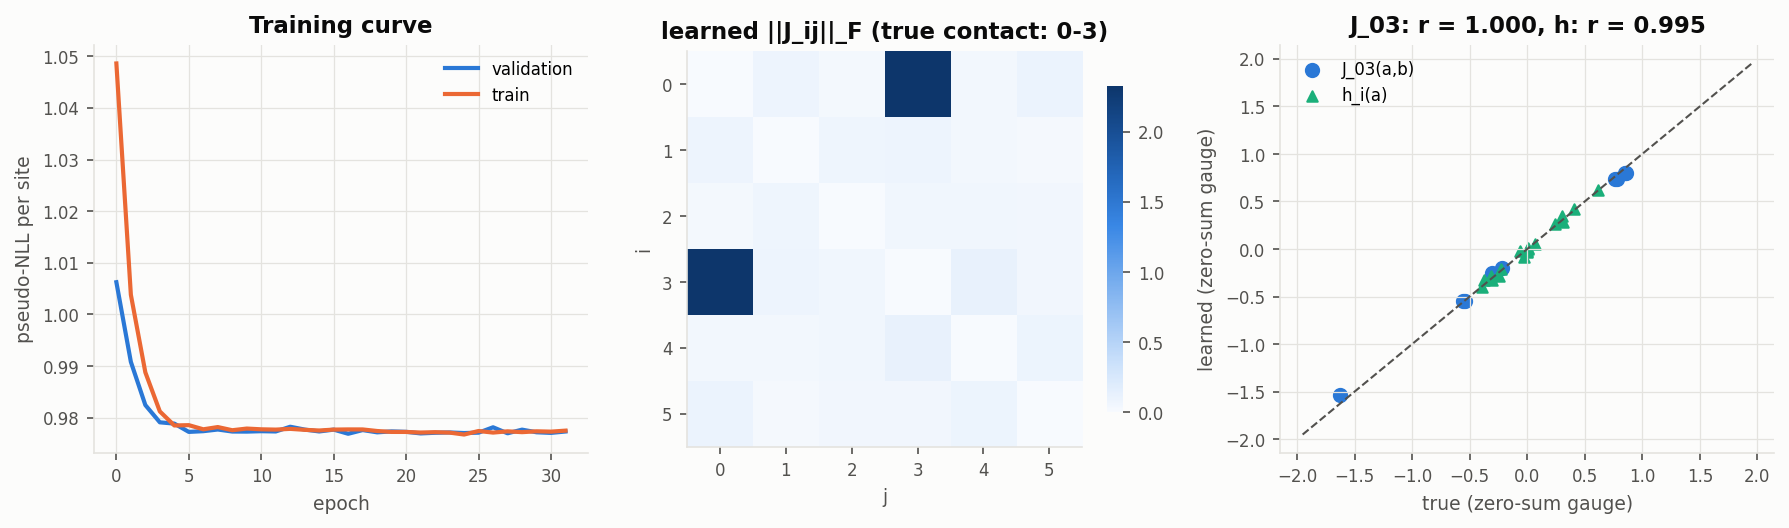
\includegraphics[width=\linewidth]{tests/test_08_factored_attention/test_learns_single_contact/toy_single_contact.png}
\caption{\texttt{test\_08}: toy model with $L=6$, $q=3$ and a single strong coupling between sites 0 and 3,
10{,}000 samples, $H=4$ heads. Left: training curve. Middle: the learned $\|J_{ij}\|$ is concentrated on
the true pair. Right: learned vs true $J_{03}(a,b)$ and $h_i(a)$ (zero-sum gauge), $r=1.000$ and $0.995$.}
\end{figure}

\begin{figure}[H]
\centering
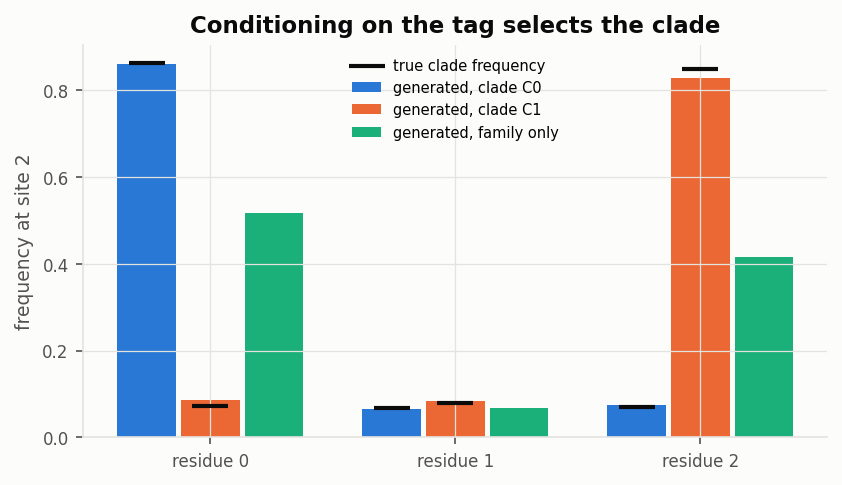
\includegraphics[width=0.62\linewidth]{tests/test_09_conditional/test_learns_clade_specific_fields/site2_by_tag.png}
\caption{\texttt{test\_09}: two clades that prefer residue 0 vs residue 2 at site 2. Sequences generated
with each clade tag reproduce that clade's frequencies (black ticks). With the clade tag dropped (family
only) the model generates the mixture.}
\end{figure}

\begin{figure}[H]
\centering
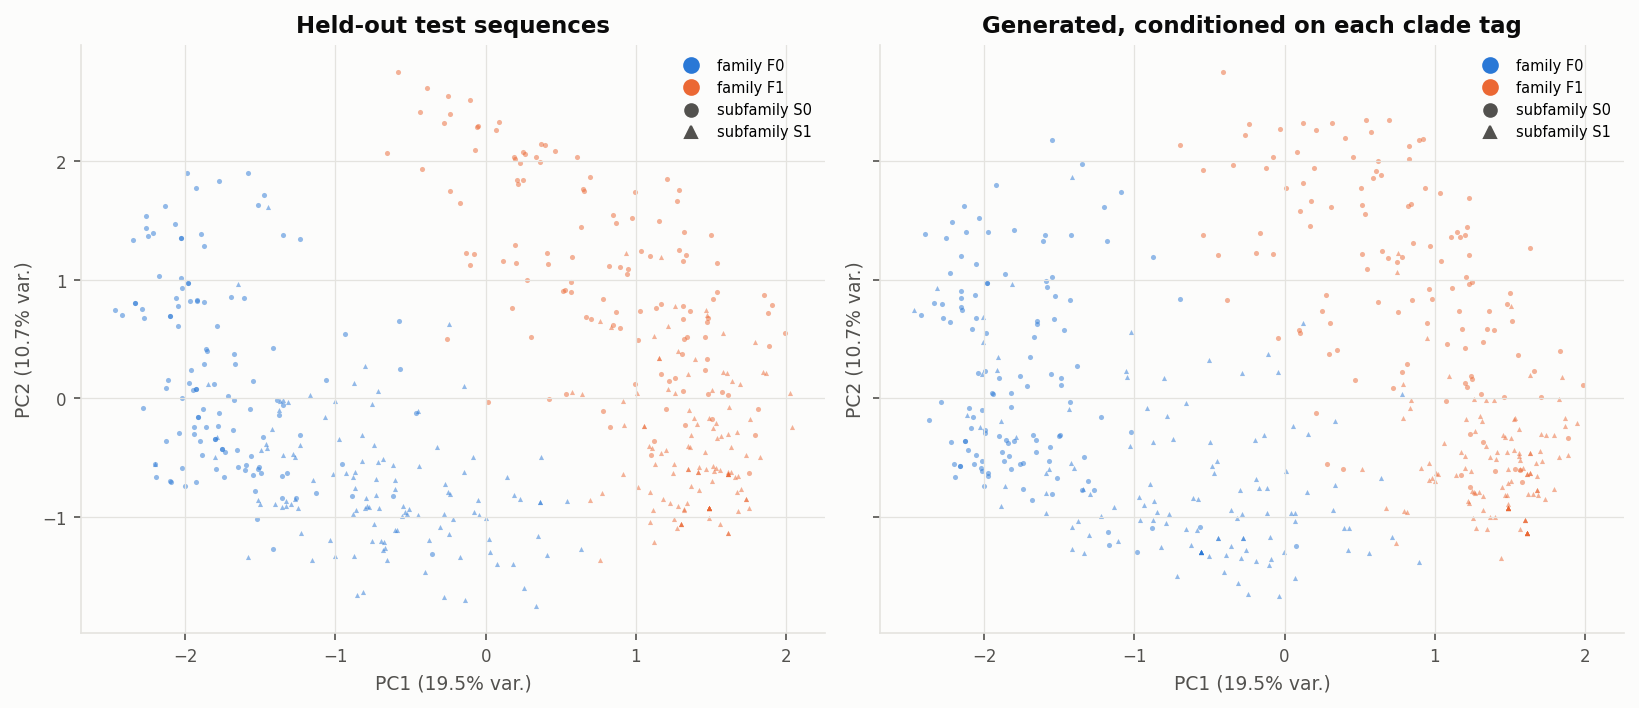
\includegraphics[width=0.9\linewidth]{tests/test_11_model_pipeline/test_model_pipeline_tiny/figures/models/tiny_conditional/pca_generated_vs_test.png}
\caption{\texttt{test\_11}: the full pipeline on a tiny tree ($L=15$, $q=5$, 8 clades) after only 4
epochs. Sequences generated with each clade tag already sit on the test sequences of their family and
subfamily on the reference PCA.}
\end{figure}

%------------------------------------------------------------------------------------------
% Results of the first trained model: unconditioned factored attention, H = 128.
% Numbers from evaluations/fa_unconditional_H128/{metrics,tree_comparison,mode_mixing}.json

\section{Results: the unconditioned model with $H=128$}\label{sec:res_uncond}

\subsection{What was trained}
The unconditioned model of \S\ref{sec:fa} was trained on all 144{,}000 training sequences (18 clades, no tags).
At your request it used $\bm{H=128}$ heads instead of the 256 of the plan, i.e.\ 543{,}920 parameters
(run \texttt{fa\_unconditional\_H128}). Note that 128 is below the $\approx179$ heads that the rank argument
of \S\ref{sec:rank} requires for an exact representation of our couplings. Everything else is as in
\S\ref{sec:plan}: pseudo-likelihood with $\lambda_h=\lambda_J=10^{-5}$, Adam ($5\times10^{-3}$), batch 512,
60 epochs. Training took 98\,s on the RTX~2060.

\begin{figure}[H]
\centering
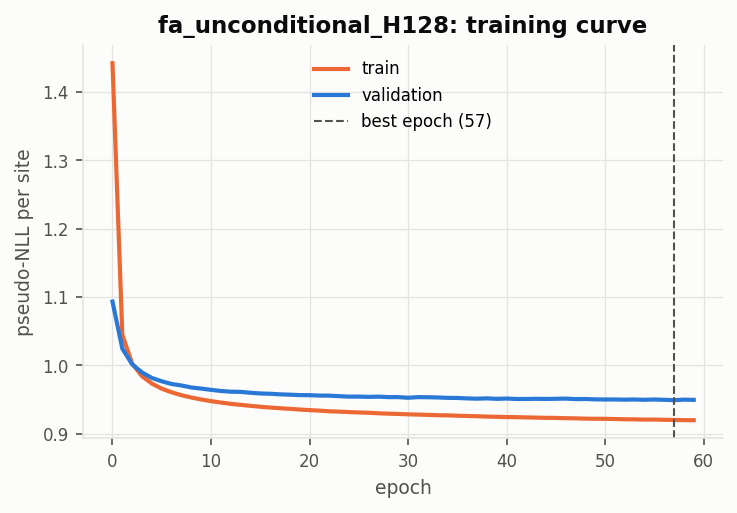
\includegraphics[width=0.55\linewidth]{models/fa_unconditional_H128/training_curve.png}
\caption{Training curve. Best validation pseudo-NLL per site: $0.949$ (epoch 57 of 60). It was still
decreasing slowly at the 60-epoch cap. The train/validation gap is small ($0.920$ vs $0.949$), so there is
little over-fitting.}
\end{figure}

For comparison (\S\ref{sec:plan}): an independent-site model scores 2.11, and the true clade models 0.80.
The unconditioned model reaches $0.95$. That is far better than independent sites, and it cannot reach
0.80, because a single Potts model cannot represent the mixture of 18 clade models.

Evaluation protocol (\S\ref{sec:evalprotocol}): 18{,}000 sequences Gibbs-sampled from the learned $(h,J)$
(200 sweeps, one sequence per chain), compared with the 18{,}000 held-out test sequences. The
\emph{oracle} is 18{,}000 fresh samples of the true clade models (1000 per clade), the best achievable score.

\subsection{Site frequencies and correlations}
\begin{center}\small
\begin{tabular}{lccccc}
\toprule
compared with the test set & $r_f$ & $r_C$ & slope $C$ & identity gen--gen & copies\\
\midrule
oracle (fresh true samples) & 1.000 & 0.994 & 0.99 & 0.197 & 0\%\\
\textbf{generated} & \textbf{0.940} & \textbf{0.895} & \textbf{0.70} & \textbf{0.260} & 0\%\\
generated, rebalanced to equal family shares$^\ast$ & 0.992 & 0.949 & 0.79 & 0.209 & 0\%\\
\bottomrule
\end{tabular}\\[2pt]
{\footnotesize $^\ast$ 2101 generated sequences from each family (see \S\ref{sec:res_props}); identity of the test set itself: 0.198.}
\end{center}

\begin{figure}[H]
\centering
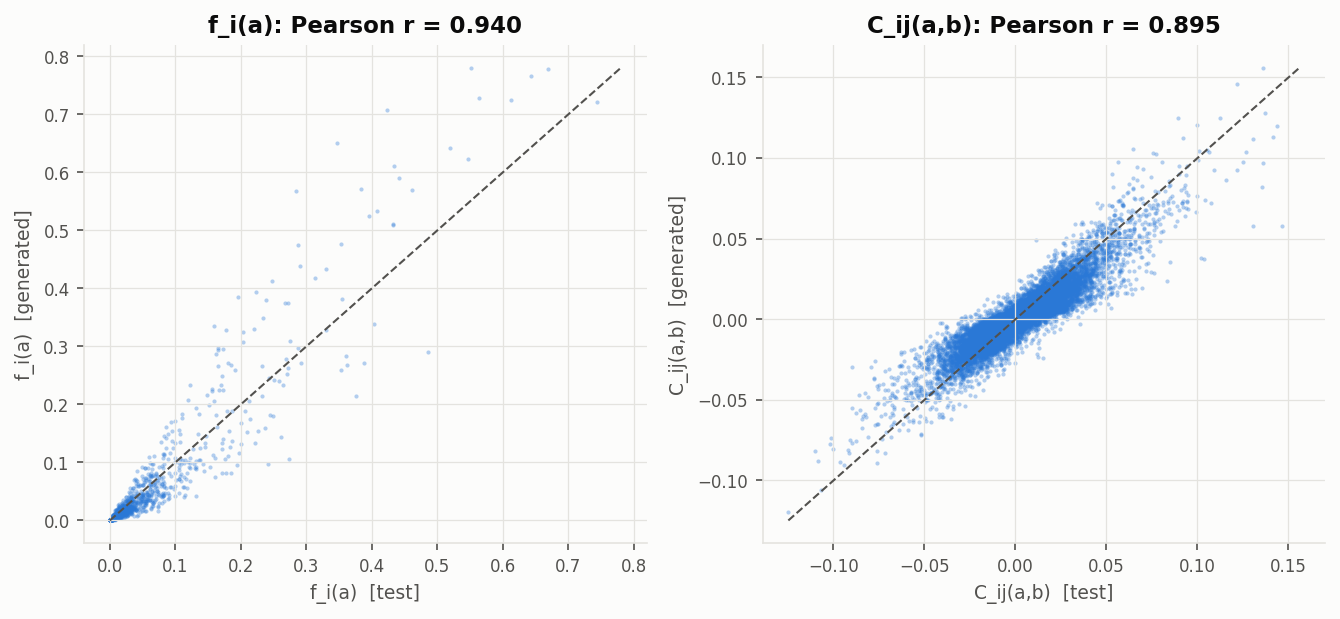
\includegraphics[width=0.49\linewidth]{models/fa_unconditional_H128/freq_corr_generated_vs_test.png}\hfill
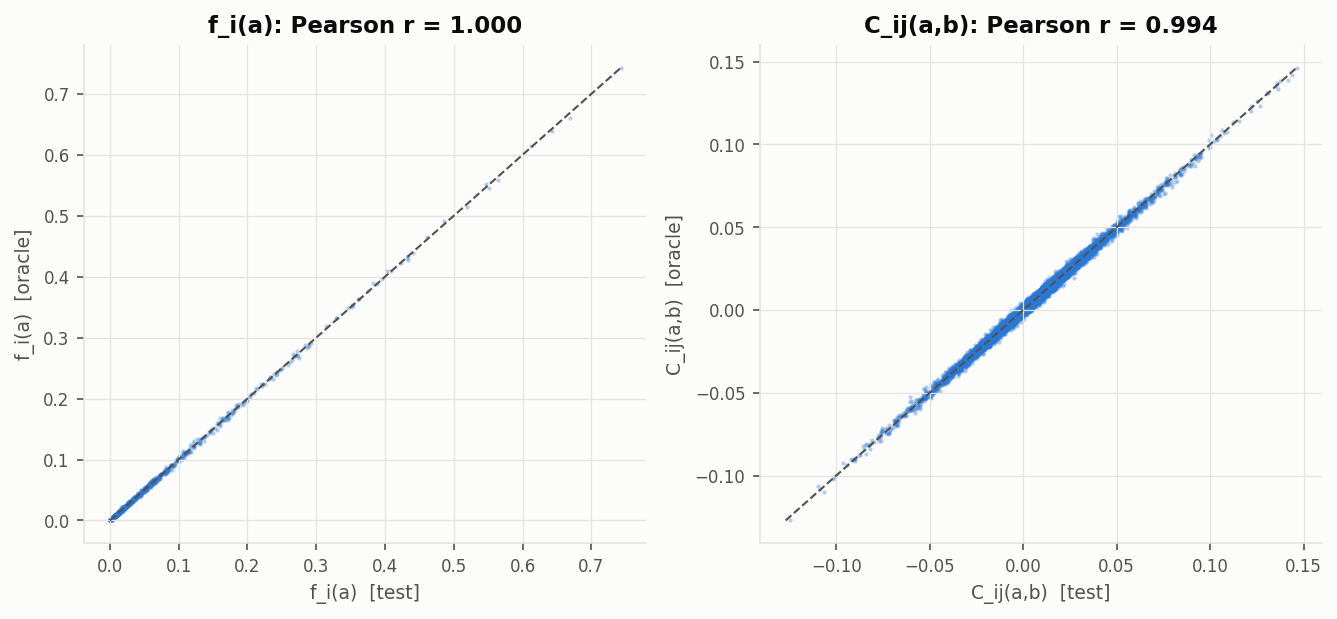
\includegraphics[width=0.49\linewidth]{models/fa_unconditional_H128/freq_corr_oracle_vs_test.png}
\caption{Site frequencies $f_i(a)$ and connected correlations $C_{ij}(a,b)$ of the generated sequences
(left pair) and of the oracle (right pair) against the test sequences. Points on the dashed line are
reproduced exactly.}
\end{figure}

\begin{figure}[H]
\centering
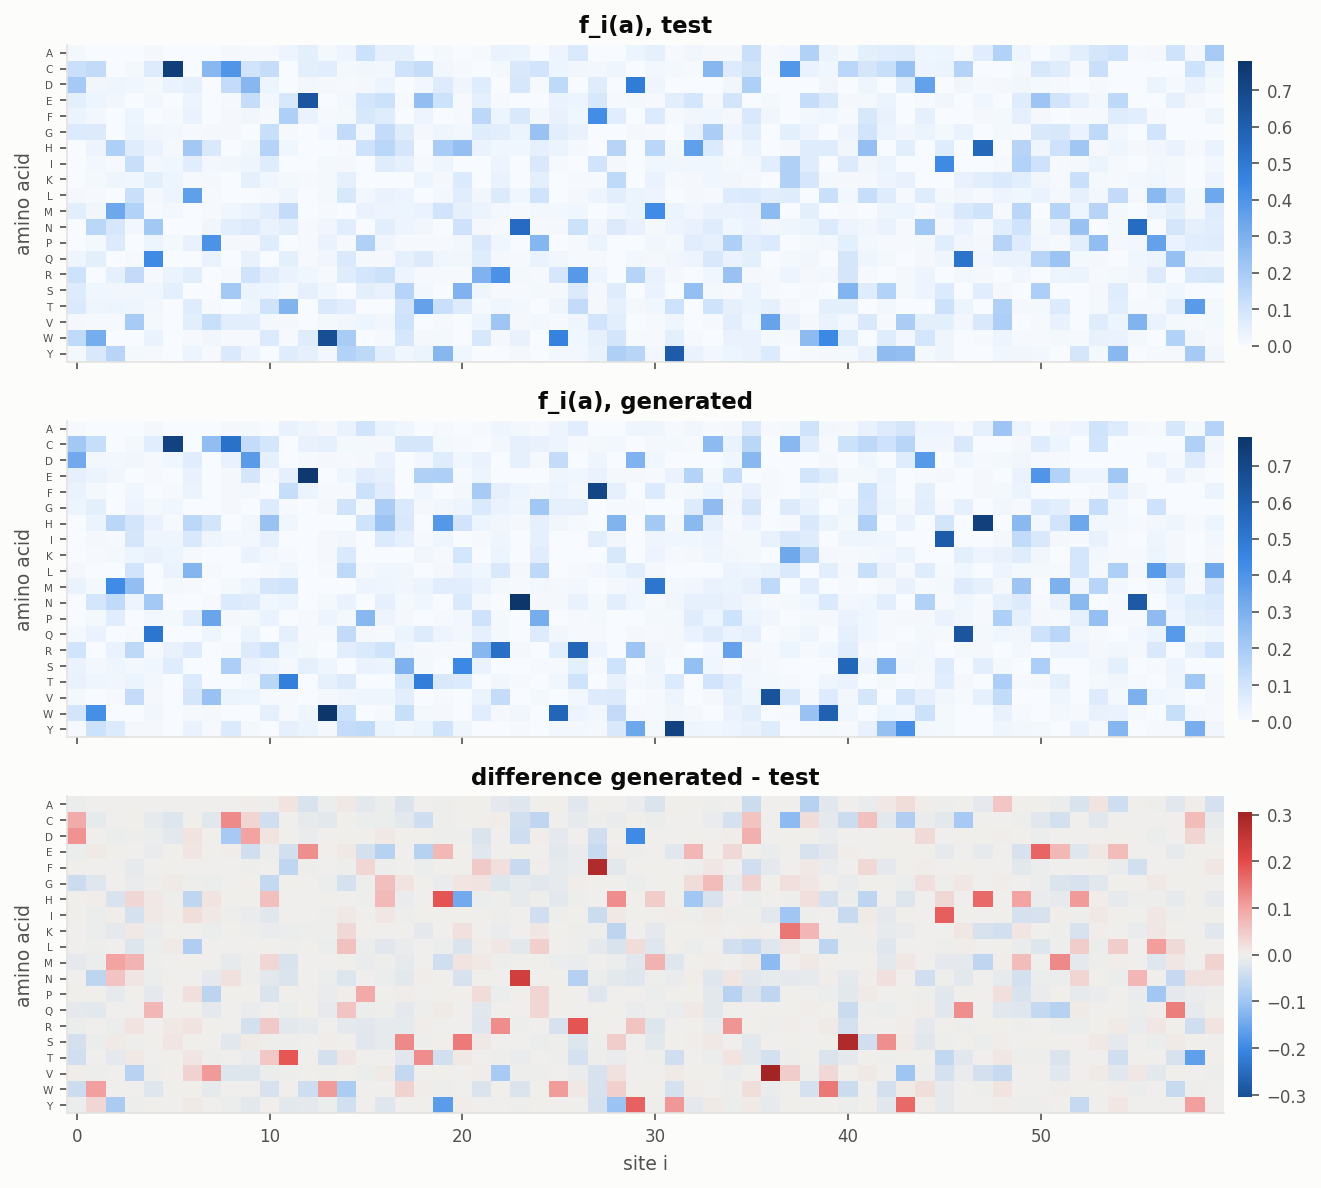
\includegraphics[width=0.78\linewidth]{models/fa_unconditional_H128/site_frequencies_test_vs_generated.png}
\caption{Site frequencies of the test set, of the generated set, and their difference (red: too frequent
in the generated sequences, blue: too rare). The errors are concentrated on a few residues at a few sites.
These are the residues that distinguish the families (next subsection).}
\end{figure}

\begin{figure}[H]
\centering
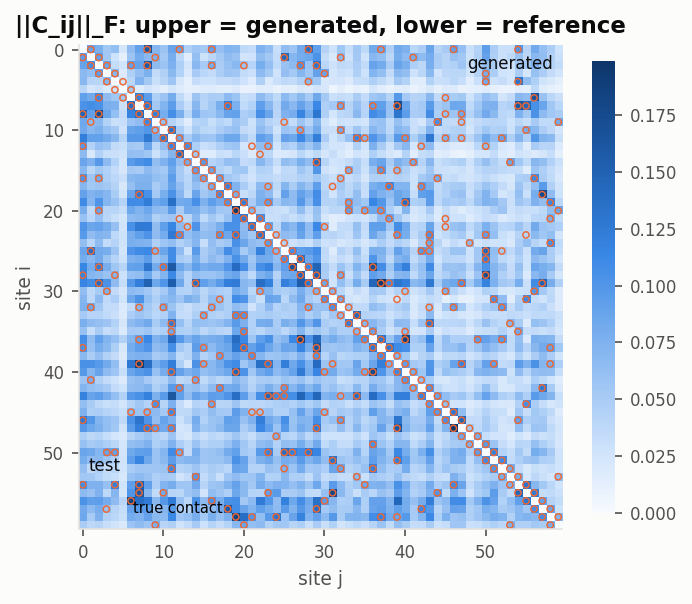
\includegraphics[width=0.5\linewidth]{models/fa_unconditional_H128/correlation_strength_test_vs_generated.png}
\caption{Strength of the correlation between every pair of sites, $\|C_{ij}\|_F$. Lower triangle: test set;
upper triangle: generated; circles: true contacts. In the \emph{pooled} data almost all pairs are correlated,
not only contacts: sites whose preferred residue differs between families become correlated through the
family identity (the mixture effect of \S\ref{sec:cond}). The generated set reproduces this background and the
strongest contact correlations.}
\end{figure}

\subsection{Family proportions: the main failure}\label{sec:res_props}
Each generated sequence is assigned to the family whose test centroid is nearest on the reference PCA (all 10
components). Sequences farther from every centroid than 99\% of the test sequences are from their own
centroid count as ``between families'' (\texttt{family\_assignment}).
\begin{center}\small
\begin{tabular}{lcccc}
\toprule
 & F0 & F1 & F2 & between\\
\midrule
test & 33.0\% & 32.7\% & 33.3\% & 1.0\%\\
oracle & 33.1\% & 32.7\% & 33.3\% & 0.9\%\\
\textbf{generated} & \textbf{21.7\%} & \textbf{11.6\%} & \textbf{66.4\%} & 0.3\%\\
\bottomrule
\end{tabular}
\end{center}

\begin{figure}[H]
\centering
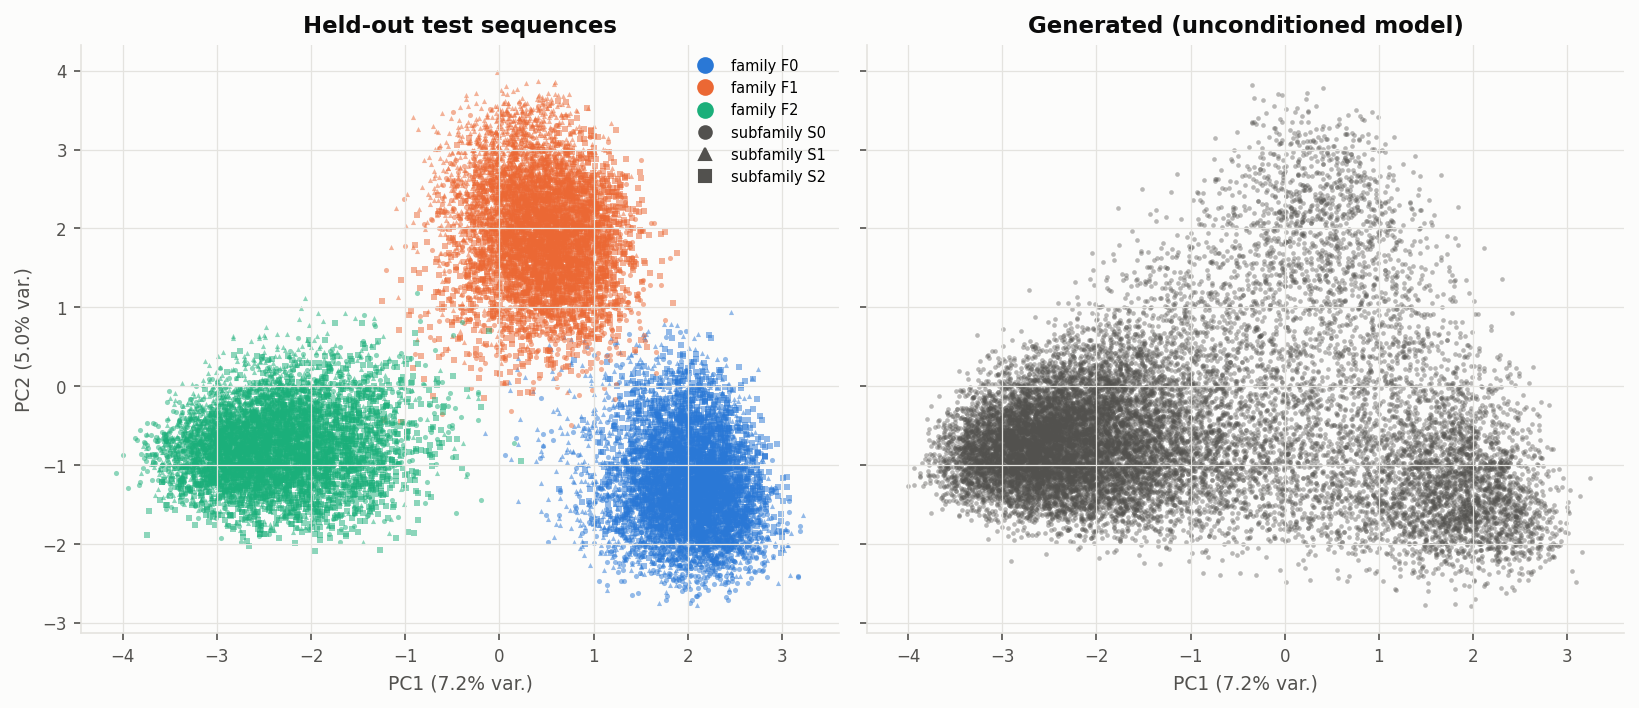
\includegraphics[width=0.85\linewidth]{models/fa_unconditional_H128/pca_generated_vs_test.png}
\caption{Test sequences (left, coloured by family) and generated sequences (right) on the reference PCA
axes of Part~I. The generated sequences occupy all three family regions, with the wrong weights: F2
(bottom left) is over-populated and F1 (top) under-populated.}
\end{figure}

\paragraph{Is it the model or the sampler?} With three well-separated families, a Gibbs chain could get
trapped in whichever family it falls into first. The proportions would then reflect the starting
points, not the learned distribution. We tested this (\texttt{s08\_mode\_mixing.py}): 600 chains were
started from random sequences, and 600 from the test sequences of each family. We then tracked where the
chains are after 100--500 sweeps.
\begin{figure}[H]
\centering
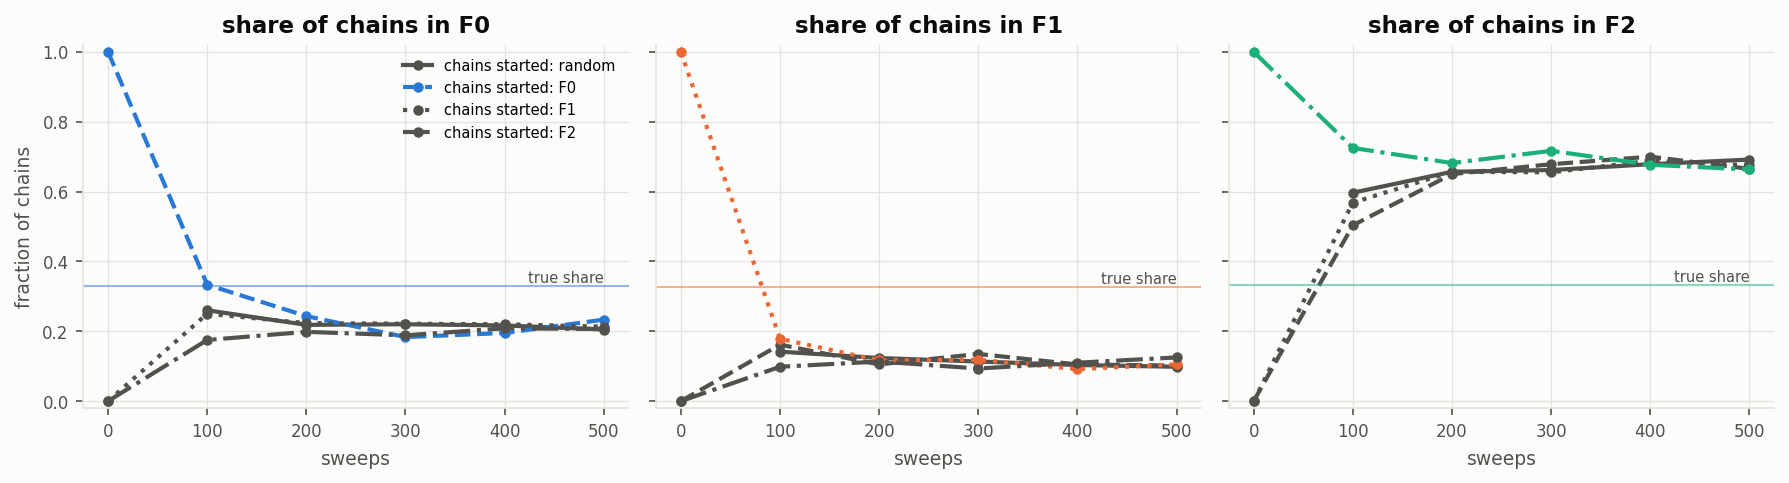
\includegraphics[width=\linewidth]{models/fa_unconditional_H128/mode_mixing.png}
\caption{Share of chains in each family vs sweeps, for chains started at random or inside F0, F1 or F2.
Chains started inside F0 or F1 leave it within 100--200 sweeps. All four starts converge to the same
$\approx20/11/68\%$ split. Horizontal lines: the true share $1/3$.}
\end{figure}
All starts converge to the same proportions, so \textbf{the sampler mixes between families and the
$20/11/68$ split is a property of the learned distribution itself.} Why would pseudo-likelihood learn wrong
family weights? The PL \eqref{eq:pl} only involves the conditionals $P(s_i\mid\s_{-i})$, which never compare
two \emph{different} regions of sequence space. The relative weight of two families is the ratio of the
total Boltzmann weight in each region, a global quantity set by $Z$, which PL never sees. As long as each
family's sequences are predicted well site by site, PL is nearly blind to how much weight each family
receives. This is a known weakness of PLM on multimodal data. The conditioned model avoids it by
construction, since the tag chooses the family.

\paragraph{Is it an energy effect? (``the sampler minimises the energy'')} Figure~\ref{fig:energytraces} shows that the clades of
F2 have the lowest mean energy, and F2 is the over-generated family, so it is natural to suspect that
sampling favours low energy. The link is real, but the mechanism is different. Two facts first:
\begin{itemize}[nosep]
\item Gibbs sampling does \emph{not} minimise the energy. It draws $\s$ with probability $e^{-E(\s)}/Z$
(validated against exact enumeration, \S\ref{sec:gibbstests}). High-energy sequences are rarer, not
excluded.
\item Figure~\ref{fig:energytraces} compares each clade under \emph{its own} model, and the clades were sampled
\emph{separately}. There the families never compete, which is why the oracle has exactly 1/3 in each.
\end{itemize}
In the learned (single) model, however, the three families do compete. The weight of family $F$ is the sum of
the Boltzmann weights of all sequences in its region:
\begin{equation}\label{eq:freeenergy}
P(F)=\frac1Z\sum_{\s\in F}e^{-E(\s)}=\frac1Z\,e^{-(\langle E\rangle_F-S_F)}
\quad\Longrightarrow\quad
\ln\frac{P(F)}{P(F')}=\underbrace{-\big(\langle E\rangle_F-\langle E\rangle_{F'}\big)}_{\text{energy term}}
+\underbrace{\big(S_F-S_{F'}\big)}_{\text{entropy term}}
\end{equation}
where $\langle E\rangle_F$ is the mean energy of the model restricted to region $F$ and $S_F$ its entropy,
i.e.\ the logarithm of the effective number of sequences in $F$. (The second equality defines $S_F$: write
$\sum_{\s\in F}e^{-E}=e^{-\langle E\rangle_F}\sum_{\s\in F}e^{-(E-\langle E\rangle_F)}$ and call the log of the
last sum $S_F$. It is exactly the Gibbs entropy of the restricted distribution.) A family can therefore win
either by having low energies or by having many sequences. We measured the energy term with 2400 samples of the
learned model and obtained the entropy term as the remainder (\texttt{s08\_mode\_mixing.py}):
\begin{center}\small
\begin{tabular}{lccccc}
\toprule
family & $\langle E\rangle_F$ & energy term & entropy term & $\ln\frac{P(F)}{P(\text{F2})}$ & site entropy\\
 & (learned model) & vs F2 & vs F2 & & (test seqs)\\
\midrule
F0 & $-176.1$ & $-10.7$ & $+9.6$ & $-1.12$ & 1.87\\
F1 & $-173.1$ & $-13.7$ & $+12.1$ & $-1.60$ & 1.94\\
F2 & $-186.8$ & 0 & 0 & 0 & 1.57\\
\bottomrule
\end{tabular}
\end{center}
F2 is the most conserved family: lowest site entropy, highest identity (0.36). Hence, in the learned model,
its sequences have $\approx11$--14 units lower energy, but its region also holds far fewer sequences. The two
effects almost cancel: an energy advantage worth a factor $e^{11}\approx60{,}000$ is reduced to a factor
$\approx3$--5 by the entropy. So \textbf{your intuition is right that the low energy of F2 is what favours it},
and it has the same origin as its low energy in Figure~\ref{fig:energytraces} (strong conservation). But the imbalance is the
small \emph{residual} of a near-cancellation between energy and entropy, not an energy minimisation. Equal
weights would need the two terms to cancel to within $\approx0.1$ nat. Pseudo-likelihood has no term that
enforces this, because the balance is a property of $Z$. That is the precise sense of the ``PL does not see
$Z$'' statement above.

\paragraph{Inside each family the sequences are good.} Taking the generated sequences assigned to each
family and comparing them with that family's test sequences:
\begin{center}\small
\begin{tabular}{lccccc}
\toprule
family & $n$ generated & $r_f$ & $r_C$ & slope $C$ & identity gen / test\\
\midrule
F0 & 3938 & 0.977 & 0.819 & 0.63 & 0.247 / 0.261\\
F1 & 2101 & 0.968 & 0.784 & 0.63 & 0.217 / 0.236\\
F2 & 11961 & 0.993 & 0.896 & 0.73 & 0.350 / 0.363\\
\bottomrule
\end{tabular}
\end{center}
The frequencies inside each family are right ($r_f\ge0.97$), and rebalancing the generated set to equal
family shares brings the pooled $r_f$ from 0.94 to 0.99 and the identity from 0.260 to 0.209 (table
above). So \textbf{most of the frequency error and most of the excess identity come from the wrong family
weights}; the remaining excess, 0.209 vs 0.198, is small. (The pooled identity was too high because F2, the most over-represented family, is also the
most internally similar one: 0.36.) What remains is that \textbf{correlations are too weak}: the slope of
generated vs test $C$ is 0.63--0.73 inside families, and 0.79 after rebalancing. This matches the shrunken
couplings found below.

\subsection{The learned $J$ compared with every $J$ of the tree}
We compare the learned couplings, in the zero-sum gauge, with each of the 31 ground-truth models. These are
the \textbf{root}, the ancestor from which all others were generated, then the 3 families, the 9 subfamilies
and the 18 clades, plus the average of the 18 clade models (\texttt{s07\_compare\_to\_tree.py}).

\begin{figure}[H]
\centering
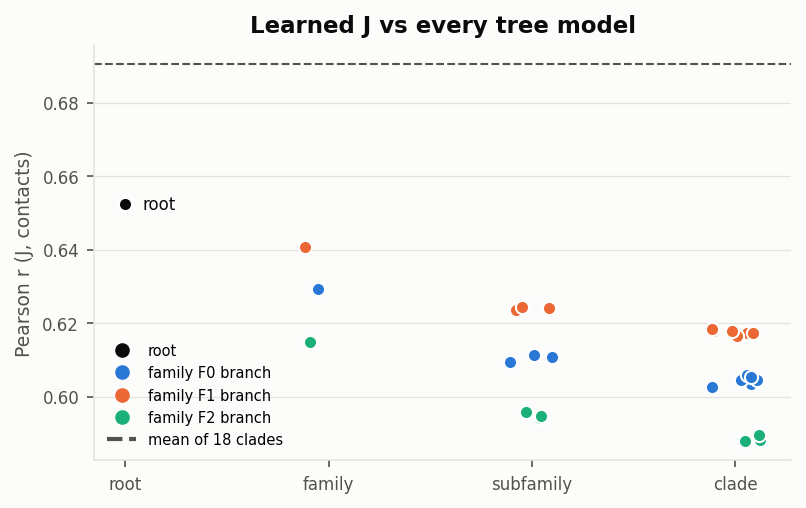
\includegraphics[width=0.49\linewidth]{models/fa_unconditional_H128/tree_rJ.png}\hfill
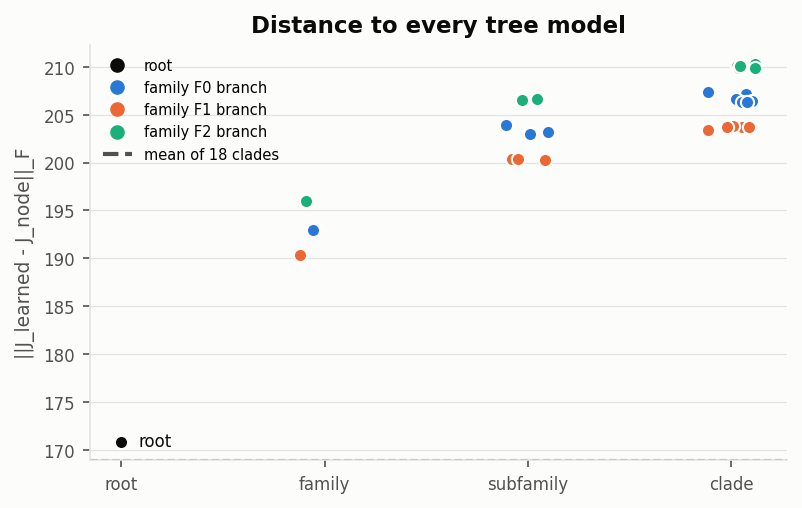
\includegraphics[width=0.49\linewidth]{models/fa_unconditional_H128/tree_dJ.png}
\caption{Learned $J$ vs every model of the tree, grouped by level, coloured by family branch. Left: Pearson
correlation on the contact entries. Right: distance $\|J^0_{\text{learned}}-J^0_{\text{node}}\|_F$. Dashed:
the average of the 18 clade models.}
\label{fig:treeJ}
\end{figure}

\begin{center}\small
\begin{tabular}{lccccc}
\toprule
compared with & $r_J$ (contacts) & slope & $d_J$ & $r_h$ & $d_h$\\
\midrule
average of the 18 clades & \textbf{0.691} & 0.57 & \textbf{168.9} & \textbf{0.922} & \textbf{26.3}\\
root (ancestor) & 0.652 & 0.57 & 170.9 & 0.865 & 27.5\\
family F0 & 0.629 & 0.48 & 192.9 & 0.836 & 36.2\\
family F1 & 0.641 & 0.49 & 190.3 & 0.857 & 35.3\\
family F2 & 0.615 & 0.47 & 196.0 & 0.802 & 39.3\\
subfamilies (range) & 0.594--0.624 & 0.43--0.46 & 200--207 & 0.78--0.84 & 38--42\\
clades (range) & 0.588--0.618 & 0.42--0.45 & 203--210 & 0.77--0.83 & 39--44\\
\bottomrule
\end{tabular}
\end{center}

\begin{figure}[H]
\centering
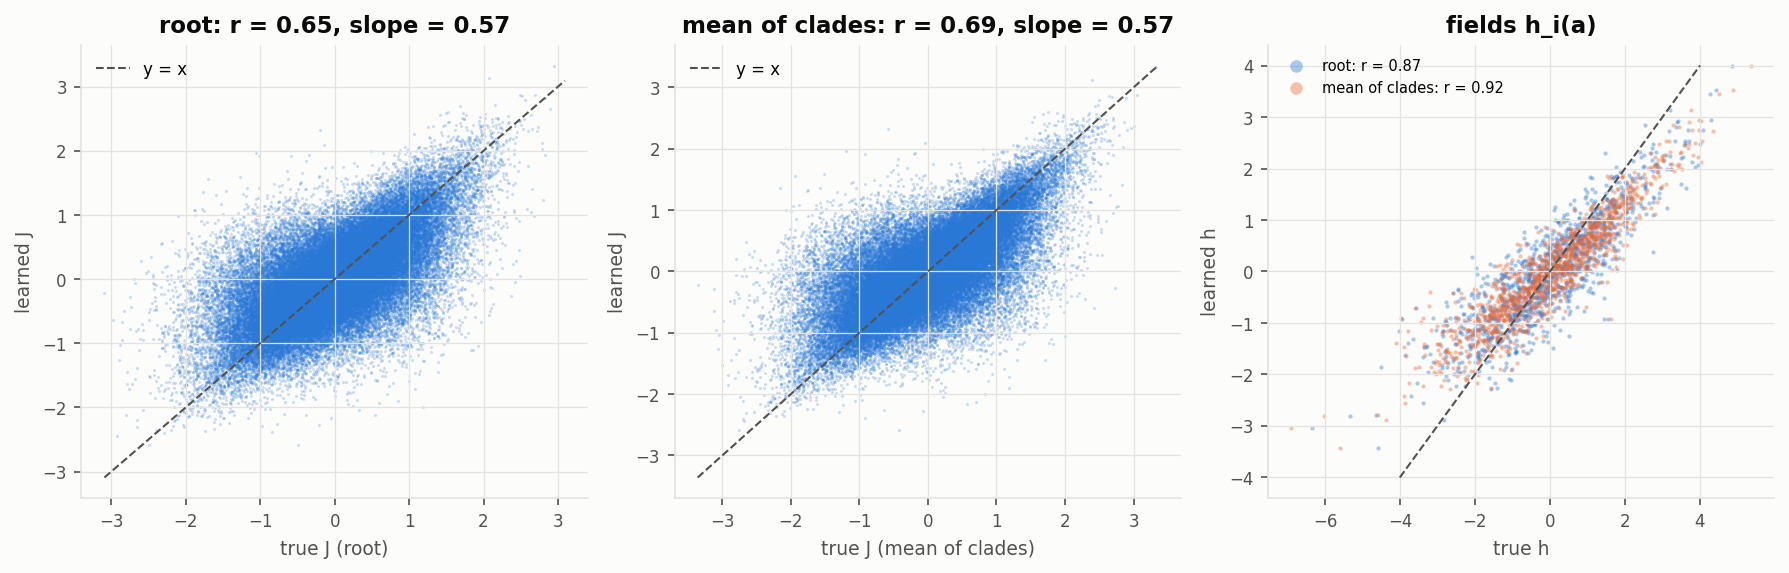
\includegraphics[width=\linewidth]{models/fa_unconditional_H128/tree_scatter_J.png}
\caption{Learned vs true couplings on the contact entries, for the root and for the average of the clades,
and learned vs true fields. The cloud is centred on a line of slope $\approx0.57$, below the diagonal.}
\end{figure}

\paragraph{Reading.}
\begin{enumerate}
\item \textbf{The model learned the common ancestor, not any family.} The similarity decreases
monotonically down the tree: root/average of clades $>$ families $>$ subfamilies $>$ clades
(Figure~\ref{fig:treeJ}). This is what one expects from fitting one Potts model to all 18 clades: the part of
$J$ shared by everyone is the ancestral part, and the family- and clade-specific perturbations average out.
The best match is the average of the clades ($r_J=0.69$), which is itself close to the root (distance 71,
against $\|J_{\text{root}}\|=202$).
\item \textbf{F2 is the \emph{least} similar family}, although it is the most over-generated. The wrong
family weights are therefore not caused by $J$ resembling F2. They sit in the global balance of $h$ and
$J$ that PL does not constrain.
\item \textbf{The couplings are too weak and partly misplaced.} The slope is 0.57: along the direction of
the true couplings, the learned ones have about 57\% of the true magnitude. This is the source of the
too-weak correlations. The distance to the root, 171, splits into 160 on the true contacts and 61 on
non-contacts, where the truth is zero but the learned model has spread couplings (mean $|J|=0.06$). The
learned contact couplings have almost the right total size (177 vs 202), but only part of them is aligned
with the true ones. The rest encodes the mixture: extra couplings that tie together the residues typical of
each family. That is exactly how a single Potts model can mimic a mixture.
\item \textbf{The contact map is found perfectly.} All 120 true long-range contacts are the 120 top-ranked
pairs by $\|J_{ij}\|$ with APC (precision $1.00$). This holds even with $H=128<179$ heads. The heads are
enough to locate every contact, though not to reproduce every coupling value.
\item The fields agree well with the average of the clades ($r_h=0.92$): conservation is learned correctly.
\end{enumerate}

\subsection{Summary of the first run}
\begin{keybox}{Unconditioned model with $H=128$}
\begin{itemize}[nosep]
\item[+] Finds all true contacts; site frequencies inside each family are right; no copies of test
      sequences; pooled correlations $r_C=0.90$ (0.95 once family shares are corrected).
\item[--] \textbf{Wrong family weights} (22/12/66\% instead of 33/33/33\%). This is a property of the
      learned distribution, not of the sampler, and is explained by pseudo-likelihood not seeing $Z$.
\item[--] Correlations about 20--35\% too weak (slope 0.63--0.79), because the couplings are shrunk
      (slope 0.57) and partly spent on representing the mixture.
\item[$\to$] Its $J$ is closest to the \emph{ancestral} (root) and \emph{average} models, and gets steadily
      further from the family, subfamily and clade models. It learned what all clades share.
\end{itemize}
Natural next steps: the conditioned model (tags fix the family weights and allow clade-specific $J$);
$H=256$ and/or more epochs to see how much of the shrinkage is capacity vs the mixture.
\end{keybox}


% Results of the conditioned model with hierarchical tags, H = 128.
% Numbers from evaluations/fa_conditional_H128/{metrics,tree_comparison,mode_mixing}.json

\section{Results: the conditioned model with $H=128$}\label{sec:res_cond}

\subsection{What was trained}
The conditioned model of \S\ref{sec:cond} (hierarchical tags, shared attention, label-specific $\Delta h$ and
$\Delta V$, hierarchical tag dropout 0.10/0.10/0.15) was trained on the same 144{,}000 sequences, with
$\bm{H=128}$ heads like the unconditioned run, so that the two differ only by the conditioning
(run \texttt{fa\_conditional\_H128}, 2{,}115{,}920 parameters, of which 1{,}572{,}000 in the label tables).
Regularisation: $\lambda_h=\lambda_J=10^{-5}$, $\lambda_{\text{label}}=10^{-4}$. Training took 23 minutes and
stopped early at epoch 47. The best epoch is 38.

\begin{figure}[H]
\centering
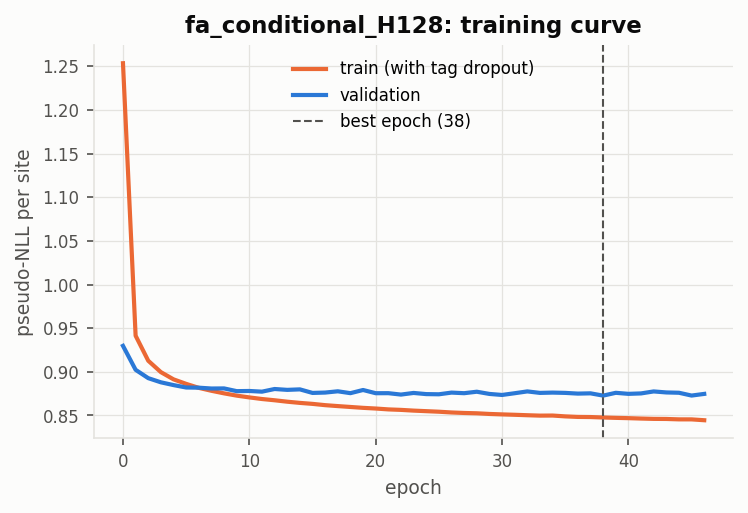
\includegraphics[width=0.55\linewidth]{models/fa_conditional_H128/training_curve.png}
\caption{Training curve. The validation pseudo-NLL (true tags) reaches $0.878$ by epoch 10 and only $0.873$
at the best epoch (38). Meanwhile the training loss keeps decreasing (with tag dropout, so it is not directly
comparable). The label tables start to fit noise beyond epoch $\approx10$.}
\end{figure}

\begin{center}\small
\begin{tabular}{lc}
\toprule
model & validation pseudo-NLL per site\\
\midrule
independent sites, one profile per clade & 1.63\\
unconditioned model ($H=128$) & 0.949\\
\textbf{conditioned model ($H=128$), true tags} & \textbf{0.873}\\
true clade Potts models (floor) & 0.80\\
\bottomrule
\end{tabular}
\end{center}
The tags close about half of the gap between the unconditioned model and the floor.

\subsection{Sequences generated with a clade tag}
For each clade, 1000 sequences were generated with its full tag and compared with that clade's 1000 test
sequences. The oracle is 1000 fresh samples of the true clade model, i.e.\ the noise floor of
\S\ref{sec:refvalues}.
\begin{center}\small
\begin{tabular}{lccccc}
\toprule
mean [min, max] over 18 clades & $r_f$ & $r_C$ & slope $C$ & identity gen / test & copies\\
\midrule
oracle & 0.998 & 0.832 [0.80, 0.88] & 0.84 & 0.337 / 0.337 & 0\%\\
\textbf{generated (clade tag)} & \textbf{0.967} & \textbf{0.758} [0.71, 0.82] & \textbf{0.75} & 0.362 / 0.337 & 0\%\\
\bottomrule
\end{tabular}
\end{center}
On the reference ladder of \S\ref{sec:refvalues} (0.83 same clade, 0.63 sibling clade, 0.35 same family,
0.08 other family), the generated clades score \textbf{0.76}. That is well above the sibling-clade level, so
the generated sequences are closer to their own clade than the true sibling clade is, but still below the
oracle. The generated sequences are slightly too similar to each other (identity 0.36 vs 0.34), and their
correlations are somewhat too weak (slope 0.75 vs 0.84 for the oracle; the oracle slope is below 1 only
because of finite-sample noise).

\begin{figure}[H]
\centering
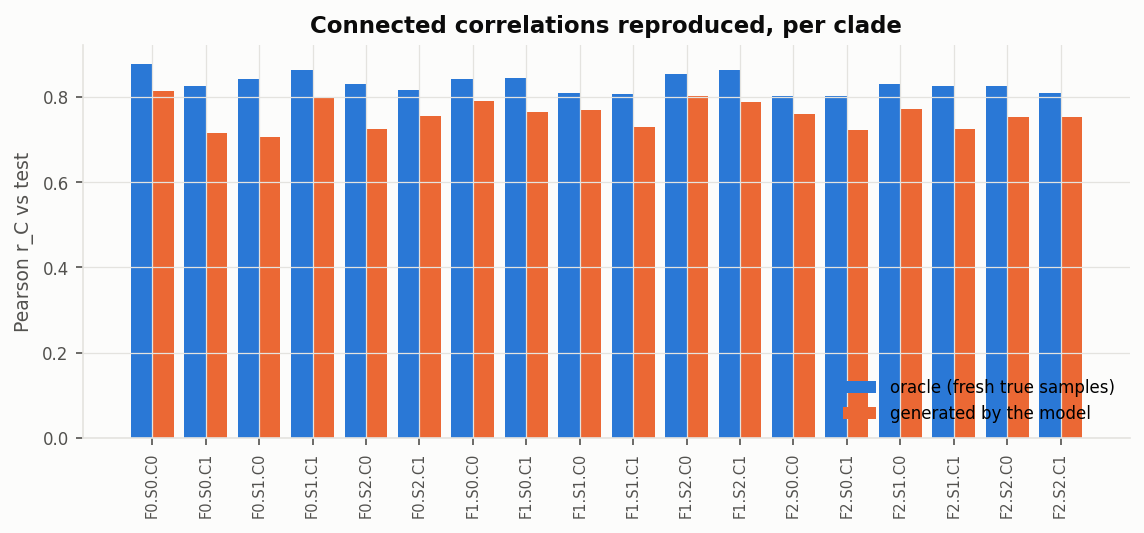
\includegraphics[width=0.8\linewidth]{models/fa_conditional_H128/rC_per_clade.png}
\caption{$r_C$ of each clade's generated sequences vs its test sequences (orange), next to the oracle (blue).
The gap is 0.04--0.14 depending on the clade.}
\end{figure}

\begin{figure}[H]
\centering
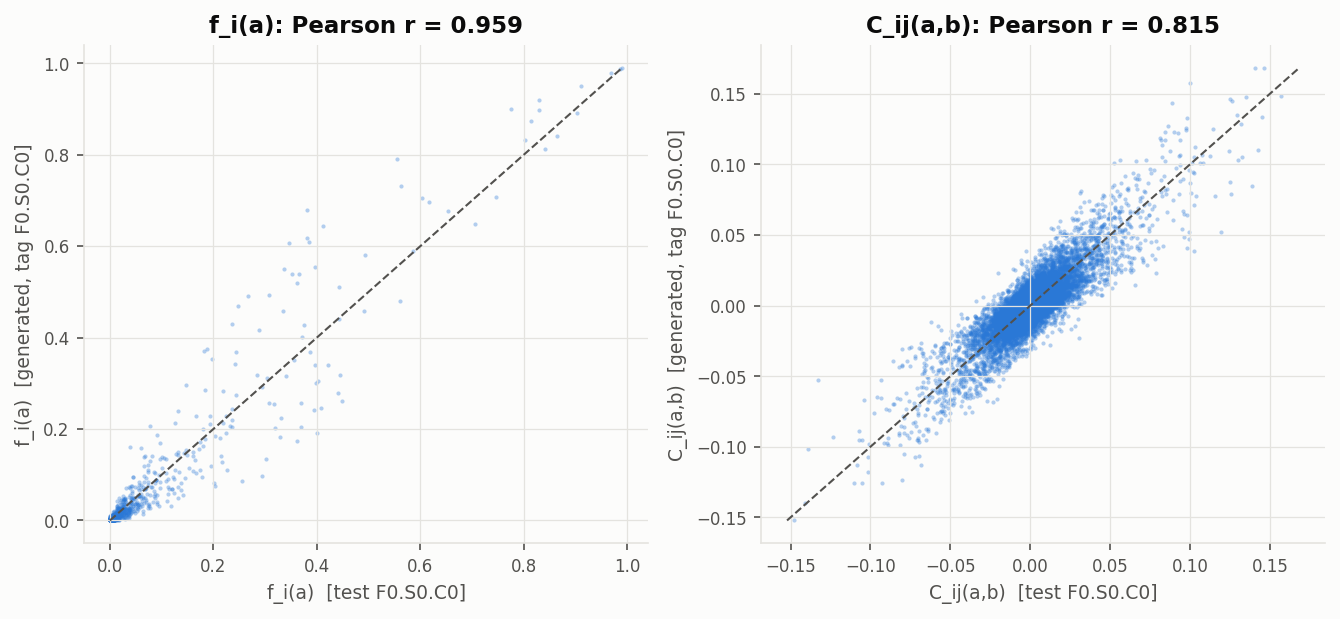
\includegraphics[width=0.49\linewidth]{models/fa_conditional_H128/freq_corr_F0.S0.C0.png}\hfill
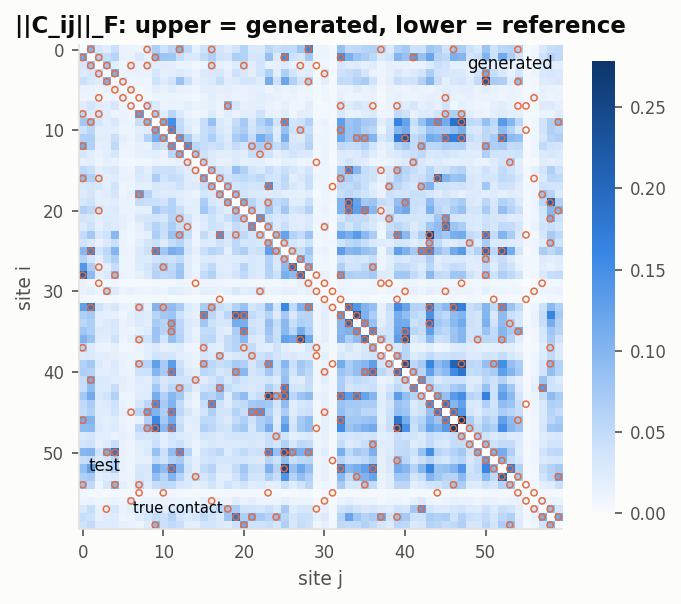
\includegraphics[width=0.4\linewidth]{models/fa_conditional_H128/correlation_strength_F0.S0.C0.png}
\caption{Example clade \texttt{F0.S0.C0}. Left: site frequencies and connected correlations, generated vs
test. Right: correlation strength $\|C_{ij}\|$, test (lower triangle) vs generated (upper), true contacts
circled. Within one clade the strongest correlations sit on true contacts. The weaker background comes from
indirect correlations and finite-sample noise (1000 sequences).}
\end{figure}

\begin{figure}[H]
\centering
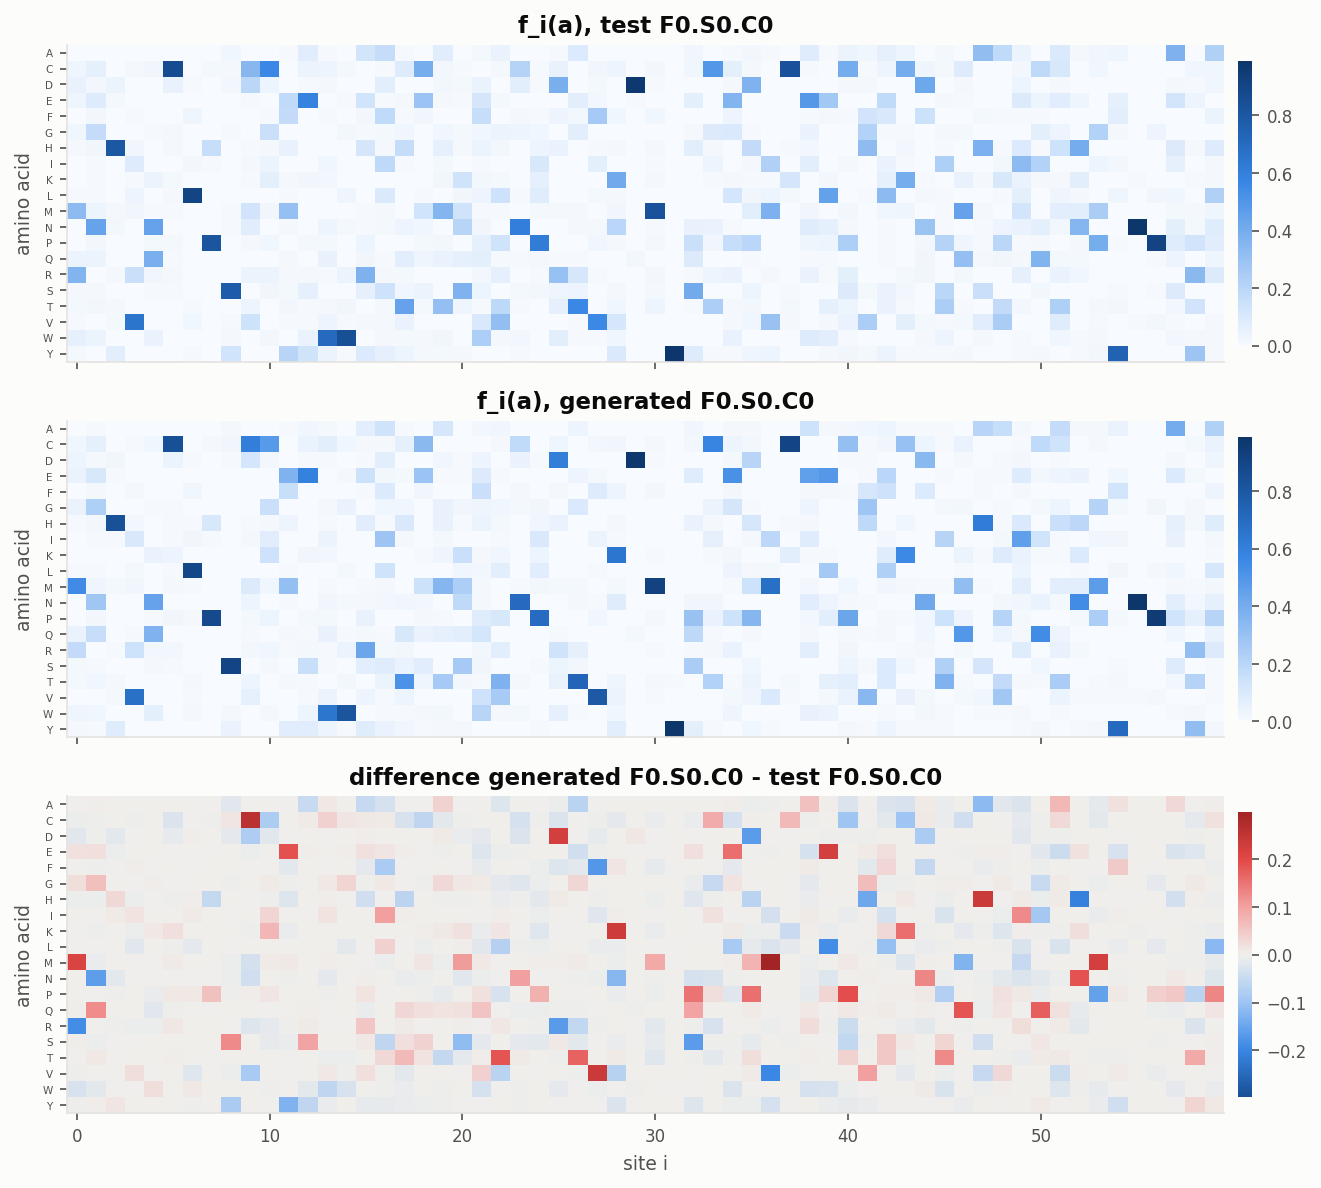
\includegraphics[width=0.78\linewidth]{models/fa_conditional_H128/site_frequencies_F0.S0.C0.png}
\caption{Site frequencies of clade \texttt{F0.S0.C0}: test, generated with its tag, and the difference.}
\end{figure}

\paragraph{Does the tag select the right clade?} For every pair (generated clade $a$, test clade $b$) we
compute $r_C$. \textbf{All 18 generated clades are closest to their own test clade} (assignment accuracy
100\%), and the matrix reproduces the hierarchy of the data: sibling clades next, then the same family.
\begin{figure}[H]
\centering
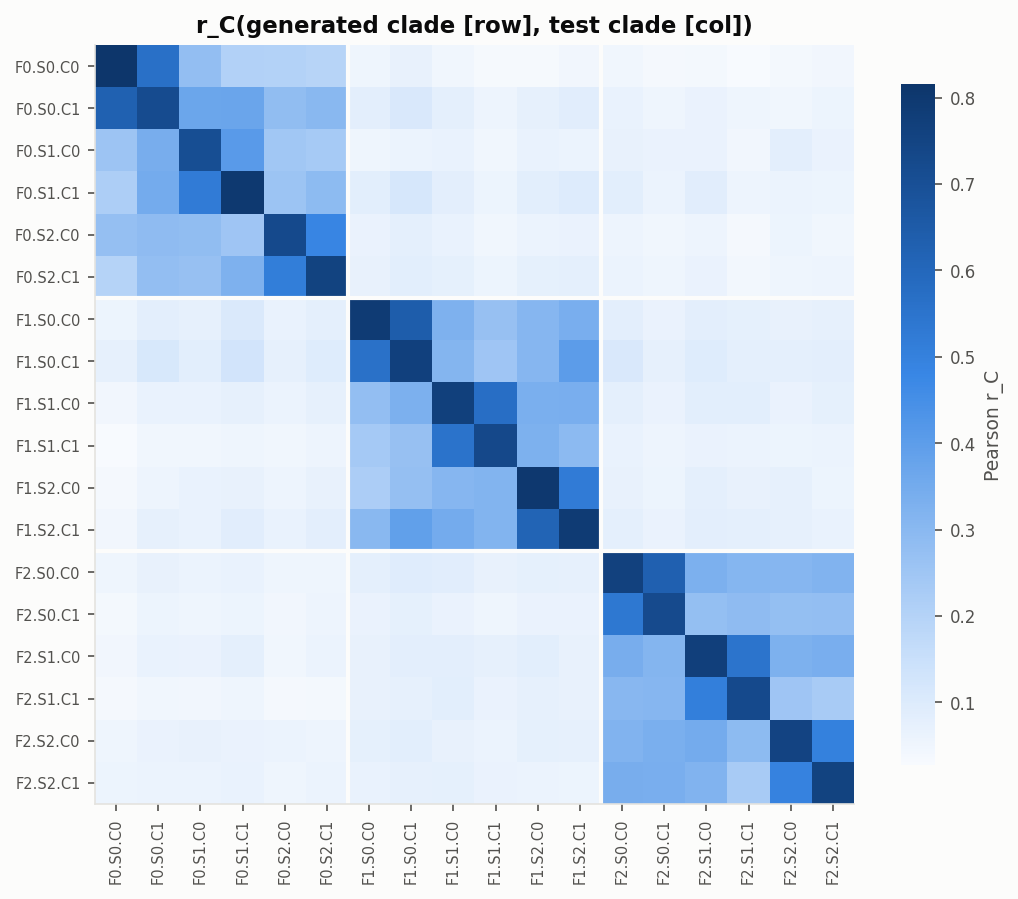
\includegraphics[width=0.62\linewidth]{models/fa_conditional_H128/cross_clade_rC.png}
\caption{$r_C$ between generated clade (row) and test clade (column). The diagonal dominates every row, and
the block structure (pairs of sibling clades, then families) is that of the ground truth.}
\end{figure}

\begin{figure}[H]
\centering
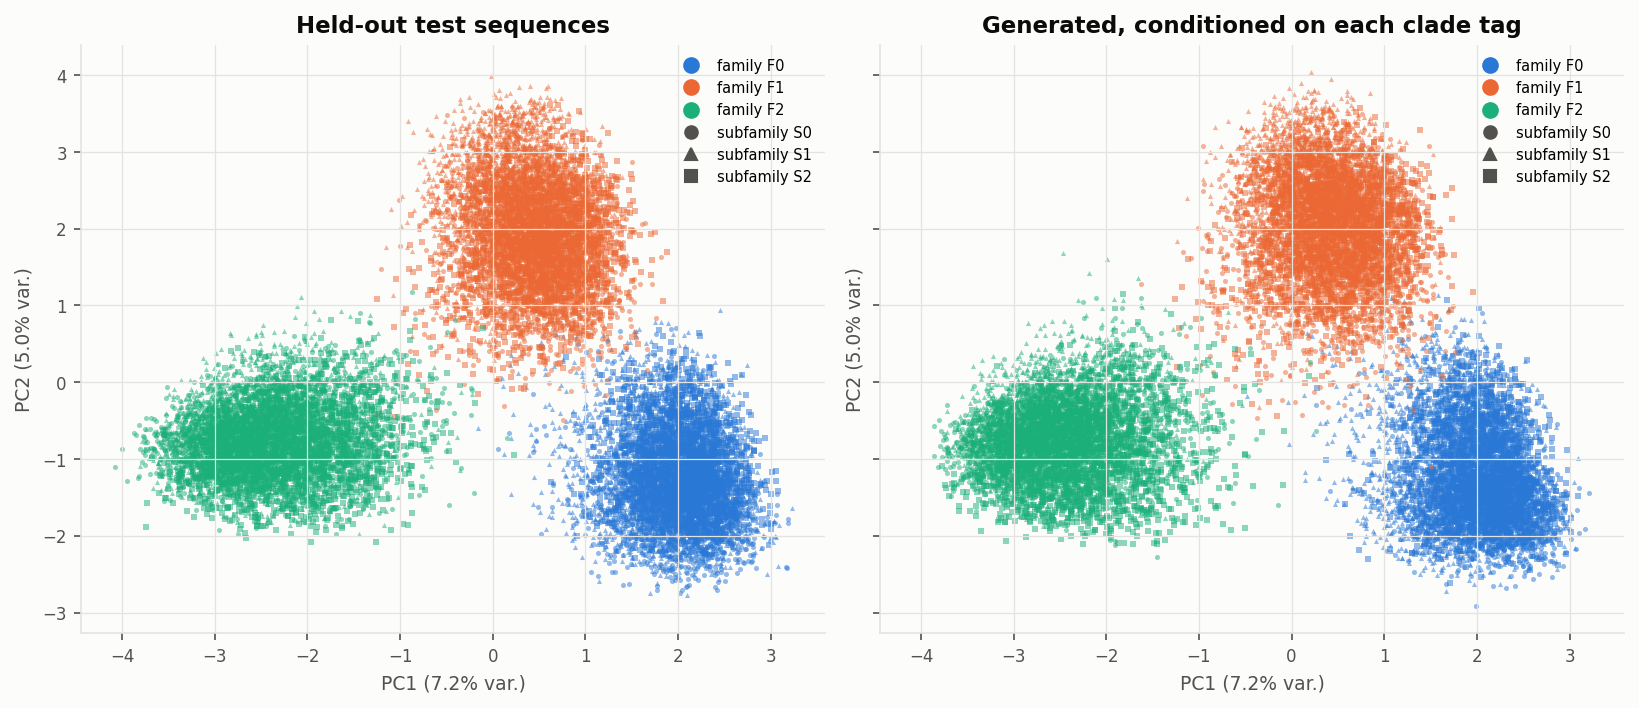
\includegraphics[width=0.85\linewidth]{models/fa_conditional_H128/pca_generated_vs_test.png}
\caption{Test sequences (left) and sequences generated with each of the 18 clade tags (right) on the reference
PCA. Pooled over the 18 tags, the generated set has exactly the right family shares (32.8/32.9/33.3\%) and
$r_f=0.992$, $r_C=0.954$ against the whole test set.}
\end{figure}

\subsection{Sequences generated with a family tag, or with no tag}
\begin{center}\small
\begin{tabular}{lccccc}
\toprule
tag & $r_f$ & $r_C$ & slope $C$ & \multicolumn{2}{c}{family of the generated sequences}\\
\midrule
family F0 only & 0.986 & 0.841 & 0.71 & \multicolumn{2}{c}{99.4\% in F0}\\
family F1 only & 0.984 & 0.856 & 0.73 & \multicolumn{2}{c}{97.8\% in F1}\\
family F2 only & 0.990 & 0.850 & 0.67 & \multicolumn{2}{c}{99.4\% in F2}\\
no tag & 0.980 & 0.872 & 0.52 & \multicolumn{2}{c}{F0/F1/F2 $=$ 33/21/46\%}\\
\bottomrule
\end{tabular}
\end{center}
(Family-tag samples are compared with the whole family's test set, 6000 sequences; no-tag samples with the
whole test set.)
\begin{itemize}
\item \textbf{A family tag generates that family}, 98--99\% of the time, with good statistics. This is
      what the unconditioned model could not do.
\item \textbf{With no tag the family weights are still wrong} (33/21/46\%), although less so than for the
      unconditioned model (22/12/66\%). This is the same pseudo-likelihood blind spot as in
      \S\ref{sec:res_props}. The no-tag mode is fitted to the whole mixture (10\% of training sequences have no
      tag). The energy/entropy breakdown (\texttt{s08}) shows the same near-cancellation as before: relative to F2, F0
      has an energy term $-9.4$ and an entropy term $+9.2$ (net $-0.27$), and F1 has $-14.1$ and $+13.3$ (net
      $-0.77$). With tags, the family weights are \emph{chosen by the user}, so this blind spot no longer matters for
      generation: pooling equal numbers of clade-tag samples gives exactly 1/3 per family (previous figure).
\end{itemize}

\subsection{The learned $J(\text{tag})$ compared with the right tensors}
Each tree node has a tag that should reproduce it: the root $\leftarrow$ no tag; family F$f$ $\leftarrow$
tag $(f,-,-)$; subfamily $\leftarrow$ family $+$ subfamily tag; clade $\leftarrow$ full tag. So we have 31
learned models for 31 true ones. Each learned $J(\text{tag})$ was compared with every true $J$
(\texttt{s07\_compare\_to\_tree.py}); the \emph{matched} comparison is the diagonal.

\begin{figure}[H]
\centering
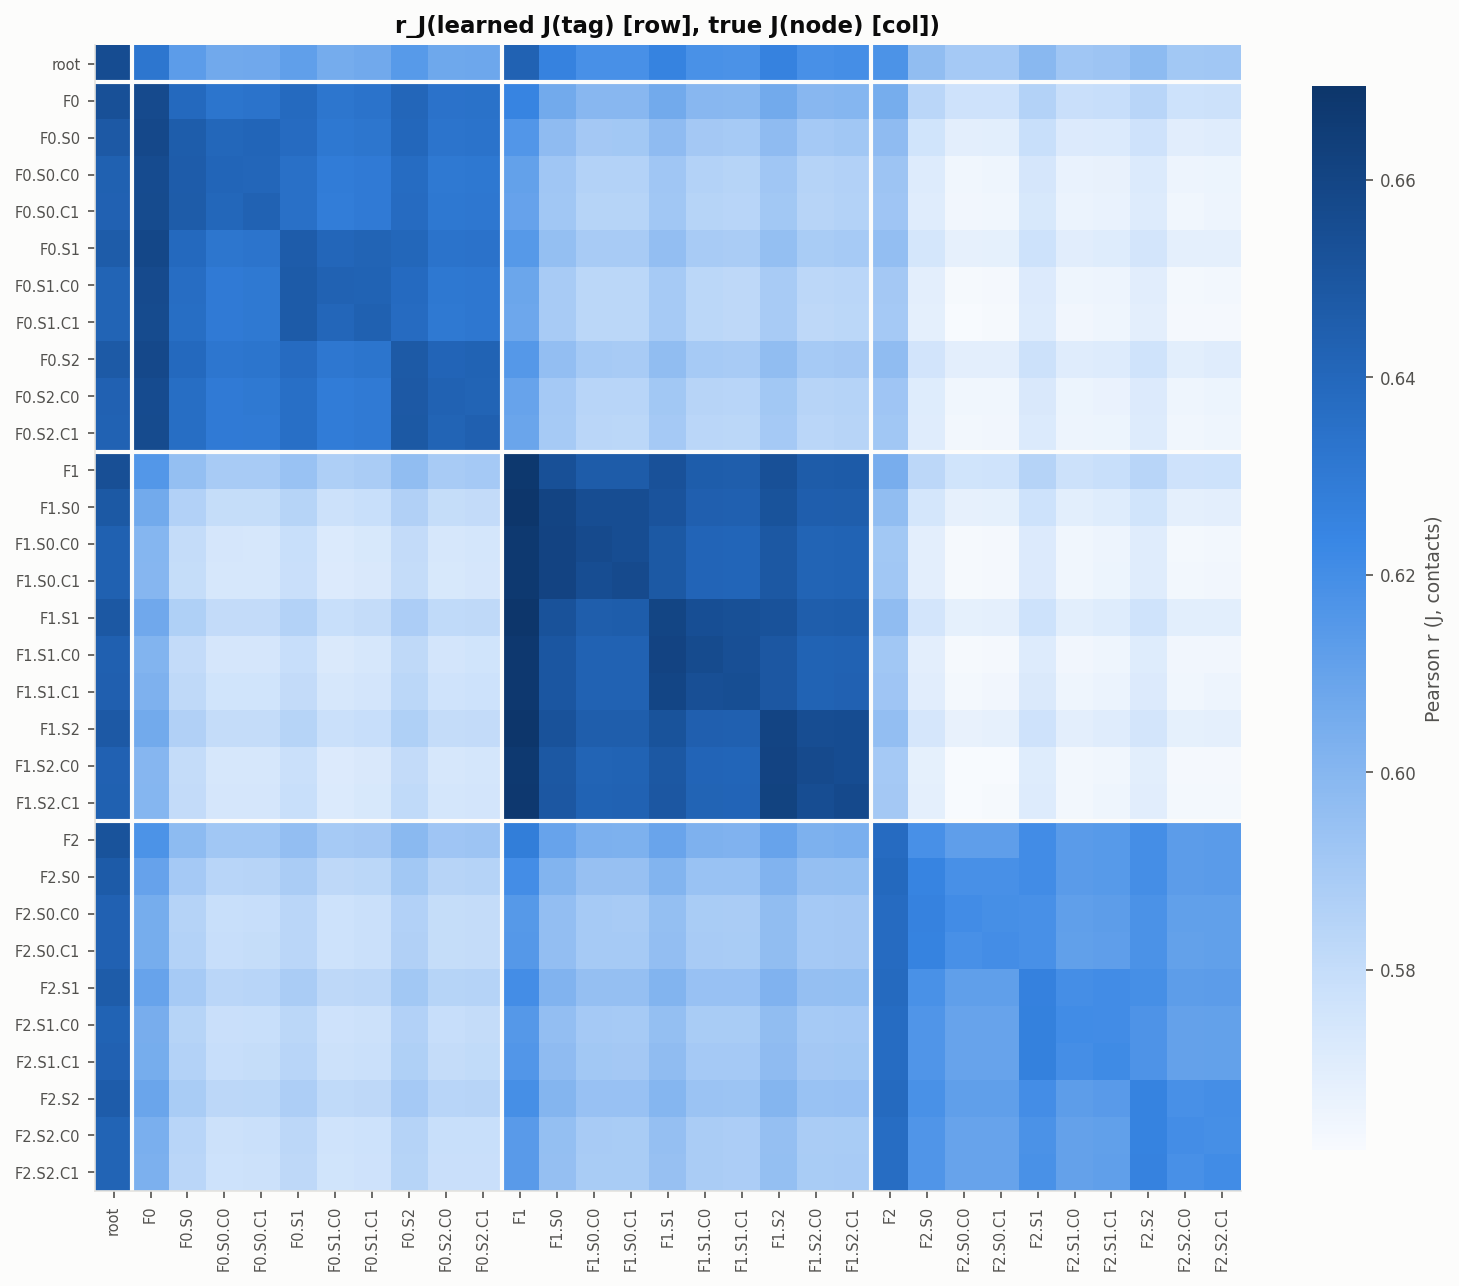
\includegraphics[width=0.8\linewidth]{models/fa_conditional_H128/tree_matrix_rJ.png}
\caption{Pearson $r_J$ (contact entries, zero-sum gauge) between the learned $J$ of each tag (rows) and every
true $J$ (columns). A perfect model would have a dark diagonal. What we see is a clear \emph{family} block
structure: every tag's $J$ resembles its own family (and the root) more than any other family. Within a
family block, however, the rows differ only slightly (a faint subfamily diagonal): the couplings barely
distinguish subfamilies and clades.}
\label{fig:matrixJ}
\end{figure}

\begin{center}\small
\begin{tabular}{lcccccc}
\toprule
level of the tag & $n$ & matched $r_J$ & matched slope & matched $r_h$ & $r(\Delta J)$ & $r(\Delta h)$\\
\midrule
none (root) & 1 & 0.655 & 0.46 & 0.871 & -- & --\\
family & 3 & 0.654 & 0.42 & 0.889 & 0.34 & 0.58\\
subfamily & 9 & 0.644 & 0.41 & 0.882 & 0.21 & 0.50\\
clade & 18 & 0.640 & 0.40 & 0.871 & 0.11 & 0.33\\
\bottomrule
\end{tabular}
\end{center}
Here $r(\Delta J)$ is the correlation between the learned change of couplings from the parent tag to the child
tag, $J(\text{child tag})-J(\text{parent tag})$, and the \emph{true} change $J_{\text{child}}-J_{\text{parent}}$
(contact entries, zero-sum gauge); $r(\Delta h)$ is the same for the fields. They measure whether the model
learned what is \emph{specific} to a label, rather than what it shares with its parent.

\begin{figure}[H]
\centering
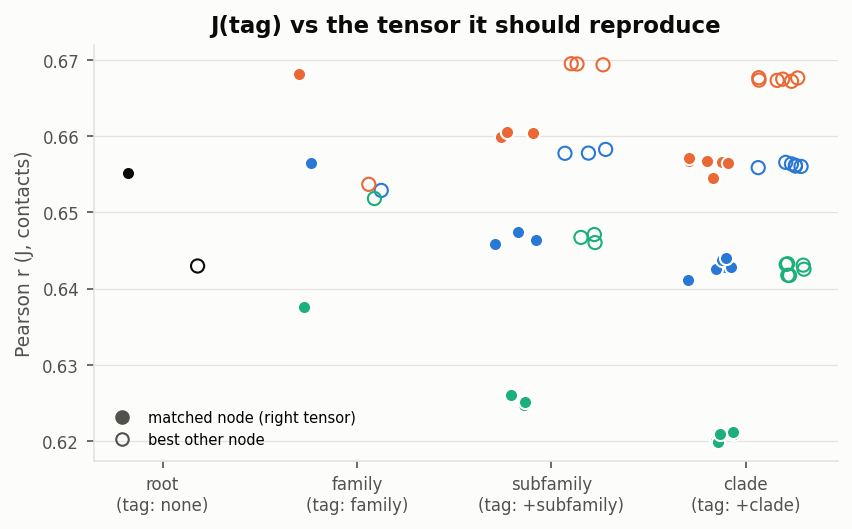
\includegraphics[width=0.55\linewidth]{models/fa_conditional_H128/tree_matched_rJ.png}
\caption{For each tag: $r_J$ with the tensor it should reproduce (filled) and with the best \emph{other} tensor
(open). At the family level the matched tensor wins for F0 and F1. At the subfamily and clade levels, another
tensor (always the tag's own family, or the root) correlates slightly better than the matched one.}
\end{figure}

By $r_J$, the true tensor that best matches each tag's $J$ is:
\begin{center}\small
\begin{tabular}{lcccc}
\toprule
level of the tag & itself & its own family & the root & another family\\
\midrule
family (3) & 2 & -- & 1 & 0\\
subfamily (9) & 0 & 6 & 3 & 0\\
clade (18) & 0 & 12 & 6 & 0\\
\bottomrule
\end{tabular}
\end{center}

\paragraph{Reading.}
\begin{enumerate}
\item \textbf{The couplings resolve the family, not the subfamily or the clade.} No tag's $J$ ever best
matches another family, but below the family level $J(\text{tag})$ is essentially the family's $J$. The
label-specific part of the couplings is weak and gets weaker with depth: $r(\Delta J)=0.34\to0.21\to0.11$.
\item \textbf{The fields carry the finer labels.} $r(\Delta h)=0.58\to0.50\to0.33$, about twice
$r(\Delta J)$ at every level. This is how the clade tags still select the right clade (100\% assignment
accuracy): the clade-specific conservation is learned in $h$.
\item \textbf{Why are the label-specific couplings weak?} Two reasons, both predictable from the architecture.
  (i) \emph{Capacity}: the label changes $J$ only through $\sum_hA^h_{ij}\Delta V^h(\text{tag})$, with the
  \emph{shared} attention and $H=128$ value matrices. The true clade perturbations are independent random blocks
  on 179 contacts, so by the rank argument of \S\ref{sec:rank} at most 128 of the 179 independent directions
  can be represented. (ii) \emph{Signal}: the true clade perturbations are small ($\sigma_J^{(3)}=0.15$, against
  0.8 for the root). Each clade tag sees only 8000 sequences, and the label tables are penalised
  ($\lambda_{\text{label}}$). The flat validation curve after epoch 10 shows that the extra label parameters
  mostly fit noise beyond that point.
\item \textbf{All couplings are shrunk.} The matched slope is $0.40$--$0.46$, i.e.\ the couplings along the
true direction are less than half their true size (0.57 in the unconditioned model). Part of the correlation
structure is instead carried by sharper fields: the generated sequences are slightly too conserved (identity
0.36 vs 0.34). Contact precision is still 1.00 for every tag.
\end{enumerate}

\subsection{Unconditioned vs conditioned}
\begin{center}\small
\begin{tabular}{p{0.36\linewidth}p{0.2\linewidth}p{0.34\linewidth}}
\toprule
 & unconditioned & conditioned (tags)\\
\midrule
validation pseudo-NLL per site & 0.949 & 0.873\\
family shares of generated sequences & 22/12/66\% & chosen by the tag (33/33/33\% pooled; 98--99\% correct per family tag)\\
$r_C$ per clade (oracle 0.83) & -- (no clade control) & 0.76\\
$r_C$ pooled (oracle 0.994) & 0.895 & 0.954\\
generated clade closest to its own test clade & -- & 18/18\\
$J$ resolves & the ancestor (root) & the family\\
long-range contact precision & 1.00 & 1.00\\
\bottomrule
\end{tabular}
\end{center}

\begin{keybox}{Conditioned model with $H=128$}
\begin{itemize}[nosep]
\item[+] Tags work: a clade tag generates its clade (18/18), a family tag its family (98--99\%), and pooling
      the tags gives the right family proportions. This removes the main failure of the unconditioned model.
\item[+] Per clade, $r_C=0.76$: between the sibling-clade level (0.63) and the noise floor (0.83).
\item[--] The learned couplings resolve only the family; subfamily and clade differences are carried mainly by
      the fields. All couplings are shrunk to $\approx40\%$ of their true size, and correlations are 10\% too weak.
\item[--] Without a tag the family weights are still off (33/21/46\%): the same pseudo-likelihood blind spot.
\end{itemize}
Levers to try next: $H=256$ (removes the rank bound on the label-specific couplings), label-specific
attention (lets tags change \emph{where} the couplings sit, not only their values), a smaller
$\lambda_{\text{label}}$ or more sequences per clade.
\end{keybox}


% Distance-based evaluation of the generated sequences (definitions in section sec:distances).
% Numbers from evaluations/<run>/metrics.json ["distances"].

\section{Results: distances between generated and real sequences}\label{sec:res_dist}
All quantities are defined in \S\ref{sec:distances}. They were computed for the four trained models; this
section reports the two $H=128$ models, and the $H=256$ models are compared in \S\ref{sec:res_H256}.

\subsection{Novelty: distance to the nearest training sequence}
\begin{center}\small
\begin{tabular}{lcccc}
\toprule
 & mean $d_{NN}$ & copies of a & $W_1$ vs & mean $d_{NN}$\\
 & to train & train seq. & test & of test seqs\\
\midrule
oracle (fresh true samples) & 0.378 & 0\% & 0.001 & 0.378\\
unconditioned, $H=128$ & 0.398 & 0\% & 0.019 & 0.378\\
conditioned, $H=128$ (per clade, mean) & 0.370 & 0\% & 0.011 & 0.378\\
\bottomrule
\end{tabular}
\end{center}
\textbf{No model copies its training data.} Not one of the 36{,}000 generated sequences equals a training sequence.
A typical held-out real sequence differs from its closest training sequence at 37.8\% of its sites
($\approx23$ of 60). The generated sequences are about as novel: the conditioned model's are marginally
\emph{closer} to the training set (0.370, i.e.\ half a site less), consistent with their slight over-conservation.
The unconditioned model's are slightly \emph{farther} (0.398). Our interpretation: a single Potts model fitted
to the mixture produces some hybrid sequences that combine features of different clades, and such sequences are
far from every training sequence.

\begin{figure}[H]
\centering
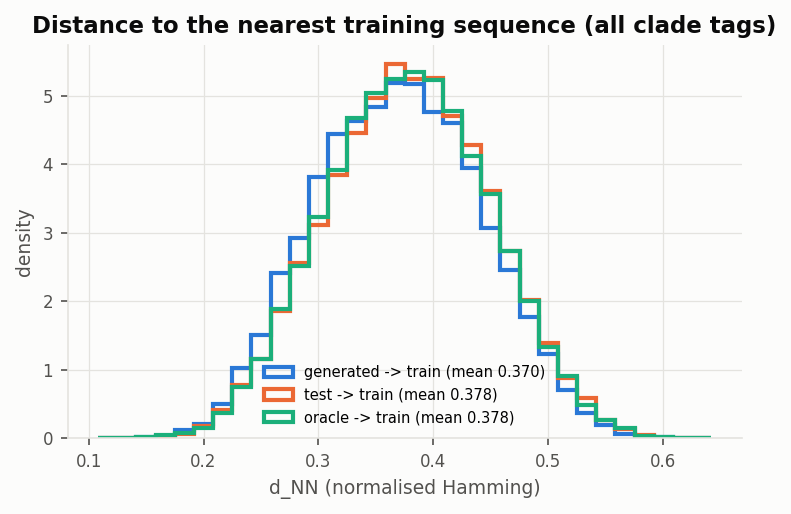
\includegraphics[width=0.49\linewidth]{models/fa_conditional_H128/dist_nn_to_train.png}\hfill
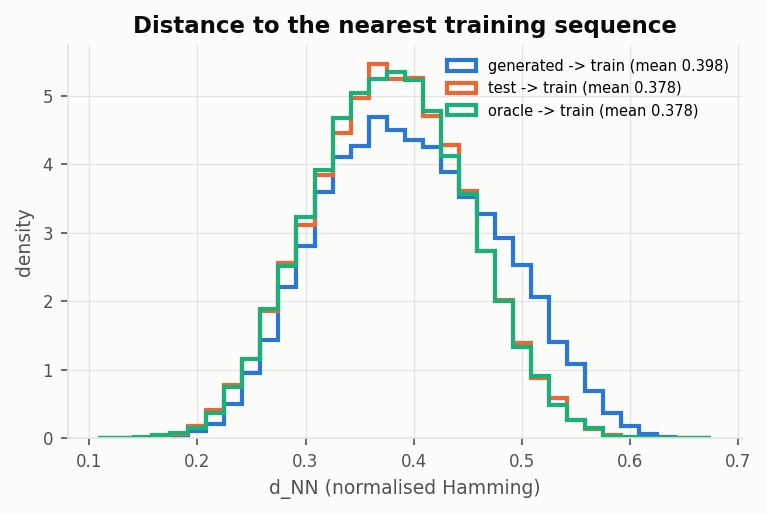
\includegraphics[width=0.49\linewidth]{models/fa_unconditional_H128/dist_nn_to_train.png}
\caption{Distribution of $d_{NN}$ to the training set. Left: conditioned model, all 18 clade tags. Right:
unconditioned model. Generated (blue), held-out test (orange), oracle (green). The oracle and test curves coincide
(same distribution); the generated curve of the conditioned model is shifted left by $\approx0.01$.}
\end{figure}

\subsection{Diversity: pairwise Hamming distances}
\begin{center}\footnotesize
\begin{tabular}{lccccc}
\toprule
 & $\bar D_{GG}$ & $\bar D_{RR}$ & $\bar D_{GR}$ & $W_1(D_{GG},D_{RR})$ & $W_1(D_{GR},D_{RR})$\\
 & (generated) & (test) & & &\\
\midrule
oracle, per clade (mean) & 0.664 & 0.663 & 0.664 & 0.003 & 0.002\\
conditioned $H=128$, per clade (mean) & 0.637 & 0.663 & 0.660 & 0.027 & 0.007\\
\midrule
oracle, pooled & 0.803 & 0.803 & 0.803 & 0.001 & 0.001\\
unconditioned $H=128$, pooled & 0.740 & 0.803 & 0.786 & 0.063 & 0.018\\
\bottomrule
\end{tabular}
\end{center}
\begin{itemize}
\item \textbf{Conditioned model.} Two sequences generated with the same clade tag differ at 63.7\% of the sites, against
66.3\% for two real sequences of that clade: 2.6\% (1.6 sites) less diversity. This is the same over-conservation
seen in the identity (0.36 vs 0.34). A generated--real pair, on the other hand, looks almost exactly like a
real--real pair ($W_1=0.007$).
\item \textbf{Unconditioned model.} The pooled diversity is clearly too low (0.740 vs 0.803). This is mostly the
wrong family weights: with 66\% of the samples in F2, most random pairs are same-family pairs, which are closer
(\S\ref{sec:res_props}).
\end{itemize}

\begin{figure}[H]
\centering
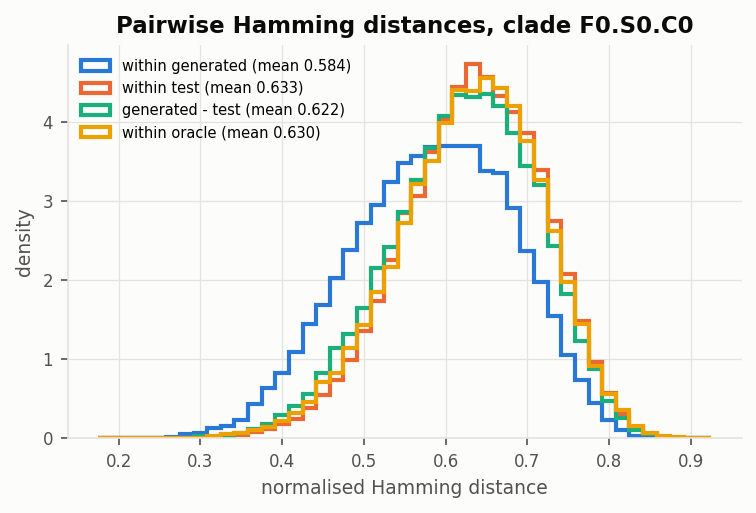
\includegraphics[width=0.49\linewidth]{models/fa_conditional_H128/dist_pairwise_F0.S0.C0.png}\hfill
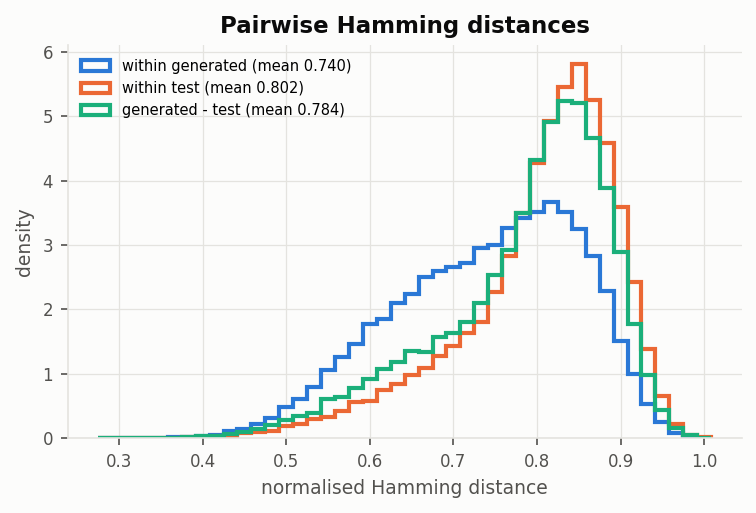
\includegraphics[width=0.49\linewidth]{models/fa_unconditional_H128/dist_pairwise.png}
\caption{Pairwise Hamming distance distributions. Left: clade \texttt{F0.S0.C0} with its tag (within generated, within
test, generated--test, within oracle). Right: unconditioned model, pooled over all clades.}
\end{figure}

\subsection{Position in PCA space: Fréchet distance}
The ladder built from the ground truth (\S\ref{sec:distances}), the Fréchet distance between the test sequences of
two clades, is
\begin{center}\small
\begin{tabular}{lcccc}
\toprule
 & same clade (oracle) & sibling clade & same family, other subfamily & other family\\
\midrule
FD (mean) & 0.02 & 1.48 & 6.15 & 21.4\\
\bottomrule
\end{tabular}
\end{center}
It spans three orders of magnitude, which makes it a sharp tool for placing a generated set in the hierarchy.
\begin{itemize}
\item \textbf{Conditioned $H=128$}: the generated clade vs its own test clade has FD $=0.39$ on average
(range 0.07--1.06). That is between the oracle (0.02) and the sibling clade (1.48). Even the worst generated clade (1.06) is closer
to its own test set than the average true sibling clade (1.48). For 17 of 18 generated clades the closest test clade
is their own (FD assignment accuracy 94\%; the $r_C$ assignment gave 18/18).
\item \textbf{Unconditioned $H=128$}, pooled: FD $=2.23$ against 0.001 for the oracle. The cloud is misplaced as a
whole because of the family weights.
\end{itemize}

\begin{figure}[H]
\centering
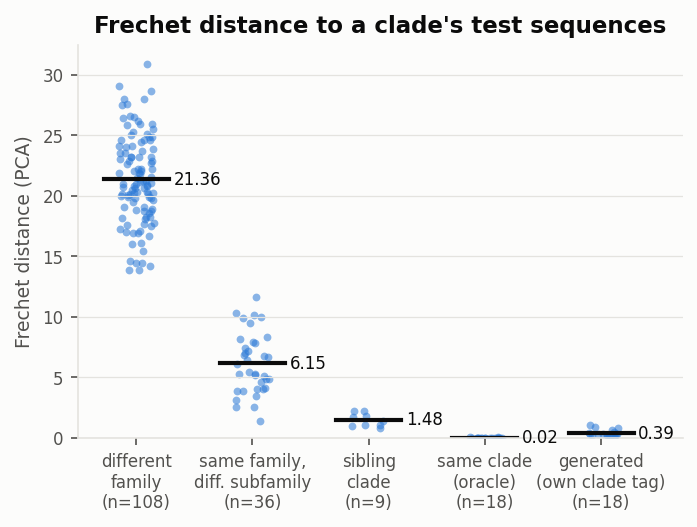
\includegraphics[width=0.49\linewidth]{models/fa_conditional_H128/frechet_ladder.png}\hfill
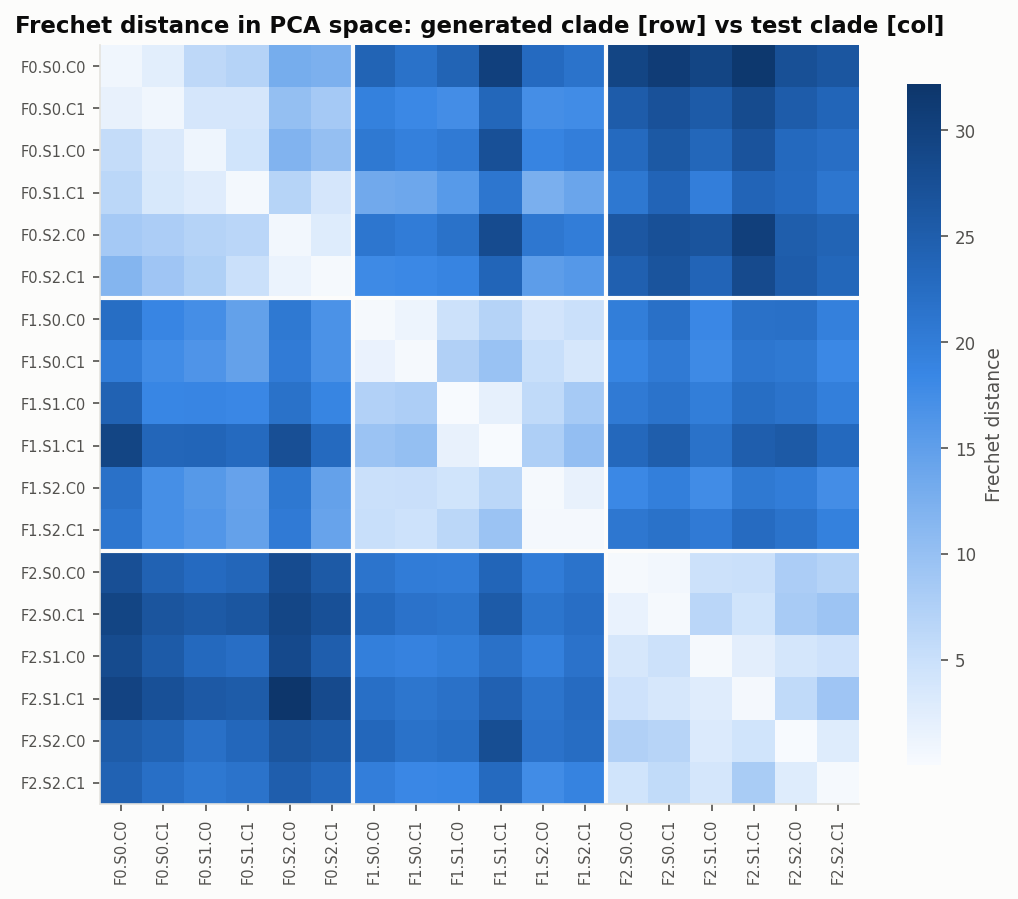
\includegraphics[width=0.49\linewidth]{models/fa_conditional_H128/cross_clade_frechet.png}
\caption{Left: FD to a clade's test sequences, for test sets of other clades grouped by relation (the ground-truth
ladder) and for the sequences generated with the clade's own tag (right-most column). Right: FD between each
generated clade (row) and each test clade (column); the dark diagonal and the family blocks are the hierarchy.}
\end{figure}

\begin{keybox}{What the distances add}
The three distance families agree with the statistics of \S\ref{sec:res_cond} and add two things:
(i) \textbf{no memorisation} (no copies, novelty equal to that of real held-out sequences); and
(ii) a \textbf{direct position in the hierarchy}: a generated clade is about 4 times closer to its own clade than
the sibling clade is (FD 0.39 vs 1.48), but 20 times farther than a perfect generator would be (0.02). Its
remaining defect is a small loss of diversity (1.6 sites), the sequence-level signature of fields that are too sharp.
\end{keybox}


% H = 128 vs H = 256 for both models.
% Numbers from evaluations/fa_{unconditional,conditional}_H{128,256}/{metrics,tree_comparison,mode_mixing}.json

\section{Results: more heads, $H=256$}\label{sec:res_H256}
Both models were retrained with $H=256$ heads, the value suggested by the rank argument of \S\ref{sec:rank}
($H\ge179$). All other settings were identical (configs \texttt{fa\_unconditional\_H256.json},
\texttt{fa\_conditional\_H256.json}; runs \texttt{fa\_*\_H256}).

\subsection{Summary table}
\begin{center}\footnotesize
\begin{tabular}{lcccc}
\toprule
 & \multicolumn{2}{c}{unconditioned} & \multicolumn{2}{c}{conditioned}\\
 & $H=128$ & $H=256$ & $H=128$ & $H=256$\\
\midrule
parameters & 0.54\,M & 1.09\,M & 2.12\,M & 4.19\,M\\
best epoch (stopped at) & 57 (60) & 36 (45) & 38 (47) & 10 (18)\\
validation pseudo-NLL / site & 0.949 & \textbf{0.946} & \textbf{0.873} & 0.888\\
\midrule
\multicolumn{5}{l}{\emph{parameters vs the ground truth (contact entries, zero-sum gauge)}}\\
$r_J$ (vs average of clades / matched clade) & 0.691 & \textbf{0.771} & 0.640 & \textbf{0.664}\\
slope of $J$ & 0.57 & \textbf{0.62} & \textbf{0.40} & 0.37\\
$r_h$ & \textbf{0.922} & 0.898 & \textbf{0.871} & 0.791\\
$r(\Delta J)$ family / subfamily / clade & -- & -- & 0.34/0.21/0.11 & 0.38/0.24/0.12\\
$r(\Delta h)$ family / subfamily / clade & -- & -- & 0.58/0.50/0.33 & 0.51/0.42/0.26\\
long-range contact precision & 1.00 & 1.00 & 1.00 & 1.00\\
\midrule
\multicolumn{5}{l}{\emph{generated sequences vs held-out test sequences}}\\
family shares (no tag) & 22/12/66\% & 11/13/76\% & 33/21/46\% & \textbf{28/31/41\%}\\
pooled $r_C$ (oracle 0.994) & \textbf{0.895} & 0.855 & \textbf{0.954} & 0.919\\
pooled $r_C$ after rebalancing & 0.949 & \textbf{0.952} & -- & --\\
per-clade $r_C$ (oracle 0.83) & -- & -- & \textbf{0.758} & 0.704\\
family-tag $r_C$ (mean) & -- & -- & 0.849 & \textbf{0.865}\\
per-clade FD in PCA space (oracle 0.02) & -- & -- & \textbf{0.39} & 0.62\\
FD assignment accuracy & -- & -- & \textbf{17/18} & 16/18\\
pairwise $\bar D_{GG}$ (test value) & 0.740 (0.803) & 0.716 (0.803) & 0.637 (0.663) & 0.633 (0.663)\\
mean $d_{NN}$ to train (test value 0.378) & 0.398 & 0.384 & 0.370 & 0.374\\
copies of training sequences & 0 & 0 & 0 & 0\\
\bottomrule
\end{tabular}
\end{center}

\subsection{Unconditioned model: better couplings, worse family weights}
With $H=256$ the learned couplings get closer to the truth ($r_J$ with the average of the clades $0.69\to0.77$,
slope $0.57\to0.62$; with the root $0.65\to0.73$). The statistics \emph{inside} each family improve (rebalanced
pooled $r_C$ 0.949 $\to$ 0.952). But the family weights get \emph{worse}: 11/13/76\% instead of 22/12/66\%. So the
pooled statistics, which include the weights, degrade ($r_C$ $0.895\to0.855$). The mixing check (\texttt{s08})
confirms again that this is the learned distribution, not the sampler: all starts converge to $\approx10/12/78\%$.
The energy/entropy decomposition \eqref{eq:freeenergy} gives an energy advantage of 13.3--13.5 for F2, compensated
by an entropy deficit of 11.6--11.8, a residual of $\approx1.8$ nats instead of 1.1--1.6.

This is a clean illustration of the pseudo-likelihood blind spot: \textbf{more capacity improves exactly what PL
measures} (each site given the others, $J$ and within-family statistics) \textbf{and does nothing for what PL
cannot see} (the relative weights of the families). A small, uncontrolled drift of the energy/entropy balance then
moves the weights further away.

\begin{figure}[H]
\centering
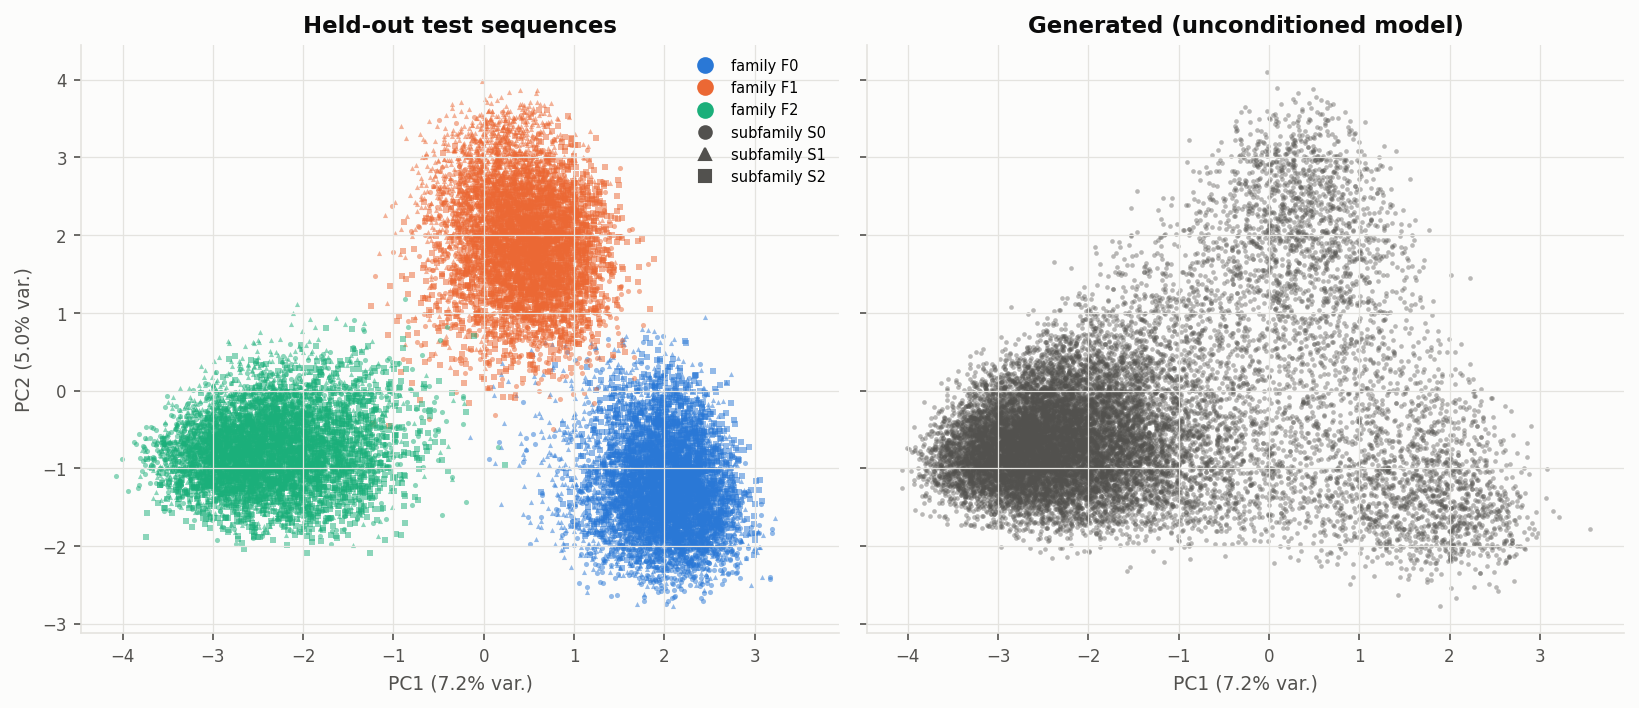
\includegraphics[width=0.85\linewidth]{models/fa_unconditional_H256/pca_generated_vs_test.png}
\caption{Unconditioned model with $H=256$: generated sequences on the reference PCA (right). F2 (bottom left) now
holds 76\% of the samples.}
\end{figure}

\subsection{Conditioned model: more heads did not help here}
The conditioned model with $H=256$ is \emph{worse} on most sequence metrics (per-clade $r_C$ $0.76\to0.70$, FD
$0.39\to0.62$), although its couplings are slightly better ($r_J$ $0.64\to0.66$, $r(\Delta J)$ slightly up at every
level). The reason is visible in the training curve. The validation loss is best at epoch 10 and does not improve afterwards, so
early stopping ended training at epoch 18. With twice the heads, the label tables hold twice as many parameters
(3.1\,M instead of 1.6\,M) under the same penalty $\lambda_{\text{label}}$. They start fitting noise within a few
epochs, before the fields have converged. The fields are indeed the component that got worse ($r_h$ $0.87\to0.79$,
$r(\Delta h)$ down at every level), and the fields are what carries the clade identity (\S\ref{sec:res_cond}).
Family-level behaviour, by contrast, improved: family tags are slightly better ($r_C$ 0.849 $\to$ 0.865) and the
no-tag family weights are closer to uniform (28/31/41\%). The mixing check confirms these weights (all starts
converge to $\approx28/31/41\%$), and the energy/entropy residual shrinks to 0.2--0.4 nats (energy terms $-9.1$ and
$-9.6$, entropy terms $+8.7$ and $+9.4$ for F0 and F1 relative to F2).

\begin{figure}[H]
\centering
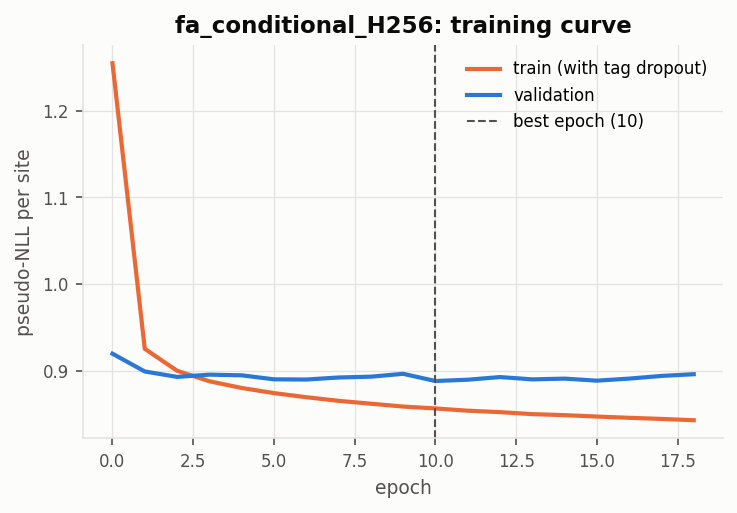
\includegraphics[width=0.49\linewidth]{models/fa_conditional_H256/training_curve.png}\hfill
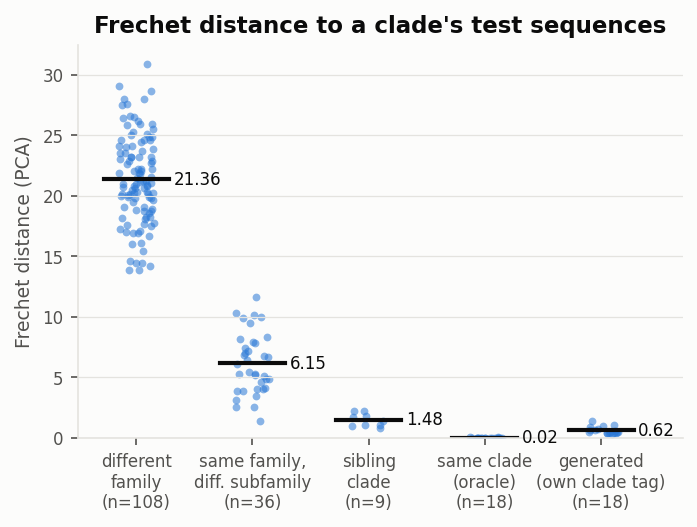
\includegraphics[width=0.49\linewidth]{models/fa_conditional_H256/frechet_ladder.png}
\caption{Conditioned model with $H=256$. Left: training curve (best epoch 10; compare the $H=128$ curve, best epoch 38).
Right: FD ladder; the generated clades (right-most column, mean 0.62) sit farther from their own clade than at
$H=128$ (0.39), still below the sibling clade (1.48).}
\end{figure}

\begin{keybox}{Conclusion on $H$}
\begin{itemize}[nosep]
\item $H=256$ recovers the couplings better in both models, as the rank argument predicts.
\item For the unconditioned model this does not translate into better samples, because its main error (family
      weights) is invisible to pseudo-likelihood and got worse.
\item For the conditioned model, the doubled label tables over-fit quickly with the current
      $\lambda_{\text{label}}=10^{-4}$, and early stopping cuts training before the fields are learned.
      $H=256$ therefore needs a stronger label penalty (or a smaller learning rate / more data per clade). As it
      stands, \textbf{the best generator is still the conditioned model with $H=128$}.
\end{itemize}
\end{keybox}


%------------------------------------------------------------------------------------------
\section{Training plan}\label{sec:plan}
%------------------------------------------------------------------------------------------
% Training plan.
\paragraph{Status.} The unconditioned model has been trained, with $H=128$ instead of 256 at your request
(results in \S\ref{sec:res_uncond}). The conditioned model has been trained with $H=128$ as well
(results in \S\ref{sec:res_cond}). Both were then retrained with $H=256$ (\S\ref{sec:res_H256}), and all four
runs were evaluated with the distance metrics of \S\ref{sec:distances} (\S\ref{sec:res_dist}).

\paragraph{Commands} (in order; all have been run, for $H=128$ and for $H=256$ with the \texttt{*\_H256.json} configs):
{\small\begin{verbatim}
python scripts/s04_make_dataset.py              # done: 144k / 18k / 18k
python scripts/s05_train_factored_attention.py --config configs/fa_unconditional.json
python scripts/s05_train_factored_attention.py --config configs/fa_conditional.json
python scripts/s06_evaluate_model.py --config configs/fa_unconditional.json
python scripts/s06_evaluate_model.py --config configs/fa_conditional.json
python scripts/s07_compare_to_tree.py --config <run config>   # J vs every tree J
python scripts/s08_mode_mixing.py --config <run config>       # model or sampler?
\end{verbatim}}

\paragraph{Hyper-parameters} (\texttt{configs/fa\_unconditional.json}, \texttt{configs/fa\_conditional.json}):
\begin{center}\small
\begin{tabular}{p{0.2\linewidth}p{0.3\linewidth}p{0.4\linewidth}}
\toprule
 & unconditioned & conditioned\\
\midrule
heads $H$, key dim $d$ & 256, 32 & 256, 32\\
parameters & 1{,}086{,}640 & 4{,}194{,}640\\
training data & all 18 clades, no tags & all 18 clades, tags with hierarchical dropout (0.10/0.10/0.15)\\
loss & PL \eqref{eq:pl} $+10^{-5}(\|h\|^2+\|J\|^2)$ & same $+\,10^{-4}\sum(\|\Delta h\|^2+\|\Delta J\|^2)$\\
optimiser & Adam, lr $5\times10^{-3}$, batch 512 & same\\
epochs & $\le60$, early stopping (patience 8) on val.\ PL & same\\
\bottomrule
\end{tabular}
\end{center}

\paragraph{Cost} (measured with 40 optimiser steps on the real data, NVIDIA RTX 2060): about
$0.2$\,min per epoch (unconditioned) and $0.4$\,min per epoch (conditioned), under 0.3\,GB of GPU memory.
That is at most $\approx12$ and $\approx25$ minutes for 60 epochs. Evaluation (Gibbs sampling of 18{,}000
sequences per model plus the oracle samples) takes a few minutes.

\paragraph{Reference values for the validation pseudo-NLL per site} (computed on the validation set):
\begin{center}\small
\begin{tabular}{lc}
\toprule
model & pseudo-NLL per site\\
\midrule
uniform residues (knows nothing) & $\log 20 = 3.00$\\
independent sites, one profile $f_i$ for all clades & 2.11\\
independent sites, one profile per clade & 1.63\\
\textbf{true clade Potts models} (the floor for the conditioned model with full tags) & \textbf{0.80}\\
\bottomrule
\end{tabular}
\end{center}
After only 40 steps the models are at 1.80 (unconditioned) and 1.53 (conditioned). The unconditioned model
cannot reach 0.80, because a single Potts model cannot represent the 18-clade mixture (\S\ref{sec:cond}). How
close it gets is itself a result.

\paragraph{What we will look at after training} (all produced by \texttt{s06}):
\begin{enumerate}[nosep]
\item training curves (\texttt{figures/models/<run>/training\_curve.png});
\item per clade: generated $r_C$ vs the oracle $r_C$ ($\approx0.83$), \texttt{rC\_per\_clade.png};
\item the cross-clade $r_C$ matrix and assignment accuracy: does the clade tag really select the clade
      rather than only its family? Compare with the reference ladder 0.83 / 0.63 / 0.35 / 0.08 of \S\ref{sec:refvalues};
\item $J$ recovery ($r_J$ on contacts) and contact precision, per clade;
\item PCA of generated vs test sequences;
\item unconditioned vs conditioned: what conditioning buys.
\end{enumerate}

\begin{checkbox}{Points to confirm before launching}
\begin{enumerate}[nosep]
\item The index reading of your formula, eq.~\eqref{eq:falogit}, together with the self-mask and the symmetrisation \eqref{eq:sym2}.
\item $H=256$ heads, from the rank argument of \S\ref{sec:rank}. Fewer heads would test whether the model can
      compress the couplings; our random ground truth predicts it cannot below $\approx179$.
\item Shared attention with label-specific values/fields in the conditioned model (\S\ref{sec:cond}). The
      alternative, label-specific $Q,K$, would let clades have different contact maps, which our ground truth does not have.
\end{enumerate}
\end{checkbox}

